\documentclass[degree=master]{thuthesis}
% 选项:
%   degree=[bachelor|master|doctor|postdoctor], % 必选
%   secret,                                     % 可选
%   pifootnote,                                 % 可选(建议打开)
%   openany|openright,                          % 可选,基本不用
%   arial,                                      % 可选,基本不用
%   arialtoc,                                   % 可选,基本不用
%   arialtitle                                  % 可选,基本不用

% 所有其它可能用到的包都统一放到这里了,可以根据自己的实际添加或者删除。
\usepackage{thuthesis}

% 定义所有的图片文件在 figures 子目录下
\graphicspath{{figures/}}

% 可以在这里修改配置文件中的定义。导言区可以使用中文。
% \def\myname{薛瑞尼}

\begin{document}

%%% 封面部分
\frontmatter
\thusetup{
  %******************************
  % 注意:
  %   1. 配置里面不要出现空行
  %   2. 不需要的配置信息可以删除
  %******************************
  %
  %=====
  % 秘级
  %=====
  secretlevel={秘密},
  secretyear={10},
  %
  %=========
  % 中文信息
  %=========
  ctitle={基于$DTW$距离测度的$Shapelet$并行算法研究},
  cdegree={工程硕士},
  cdepartment={软件学院},
  cmajor={软件工程},
  cauthor={姜友友},
  csupervisor={邓仰东副教授},
  %cassosupervisor={陈文光教授}, % 副指导老师
  %ccosupervisor={某某某教授}, % 联合指导老师
  % 日期自动使用当前时间,若需指定按如下方式修改:
  % cdate={超新星纪元},
  %
  % 博士后专有部分
  cfirstdiscipline={计算机科学与技术},
  cseconddiscipline={系统结构},
  postdoctordate={2009年7月——2011年7月},
  id={编号}, % 可以留空: id={},
  udc={UDC}, % 可以留空
  catalognumber={分类号}, % 可以留空
  %
  %=========
  % 英文信息
  %=========
  etitle={Research on Parallel Shapelet Algorithm Based on DTW Distance},
  % 这块比较复杂,需要分情况讨论:
  % 1. 学术型硕士
  %    edegree:必须为Master of Arts或Master of Science(注意大小写)
  %             “哲学、文学、历史学、法学、教育学、艺术学门类,公共管理学科
  %              填写Master of Arts,其它填写Master of Science”
  %    emajor:“获得一级学科授权的学科填写一级学科名称,其它填写二级学科名称”
  % 2. 专业型硕士
  %    edegree:“填写专业学位英文名称全称”
  %    emajor:“工程硕士填写工程领域,其它专业学位不填写此项”
  % 3. 学术型博士
  %    edegree:Doctor of Philosophy(注意大小写)
  %    emajor:“获得一级学科授权的学科填写一级学科名称,其它填写二级学科名称”
  % 4. 专业型博士
  %    edegree:“填写专业学位英文名称全称”
  %    emajor:不填写此项
  edegree={Master of Engineering},
  emajor={Software Engineering},
  eauthor={Jiang Youyou},
  esupervisor={Associate Professor Deng Yangdong},
  %eassosupervisor={Chen Wenguang},
  % 日期自动生成,若需指定按如下方式修改:
  % edate={December, 2005}
  %
  % 关键词用“英文逗号”分割
  ckeywords={\TeX, \LaTeX, CJK, 模板, 论文},
  ekeywords={\TeX, \LaTeX, CJK, template, thesis}
}

% 定义中英文摘要和关键字
\begin{cabstract}
  论文的摘要是对论文研究内容和成果的高度概括。摘要应对论文所研究的问题及其研究目
  的进行描述,对研究方法和过程进行简单介绍,对研究成果和所得结论进行概括。摘要应
  具有独立性和自明性,其内容应包含与论文全文同等量的主要信息。使读者即使不阅读全
  文,通过摘要就能了解论文的总体内容和主要成果。

  论文摘要的书写应力求精确、简明。切忌写成对论文书写内容进行提要的形式,尤其要避
  免“第 1 章……;第 2 章……;……”这种或类似的陈述方式。

  本文介绍清华大学论文模板 \thuthesis{} 的使用方法。本模板符合学校的本科、硕士、
  博士论文格式要求。

  本文的创新点主要有:
  \begin{itemize}
    \item 用例子来解释模板的使用方法;
    \item 用废话来填充无关紧要的部分;
    \item 一边学习摸索一边编写新代码。
  \end{itemize}

  关键词是为了文献标引工作、用以表示全文主要内容信息的单词或术语。关键词不超过 5
  个,每个关键词中间用分号分隔。(模板作者注:关键词分隔符不用考虑,模板会自动处
  理。英文关键词同理。)
\end{cabstract}

% 如果习惯关键字跟在摘要文字后面,可以用直接命令来设置,如下:
% \ckeywords{\TeX, \LaTeX, CJK, 模板, 论文}

\begin{eabstract}
   An abstract of a dissertation is a summary and extraction of research work
   and contributions. Included in an abstract should be description of research
   topic and research objective, brief introduction to methodology and research
   process, and summarization of conclusion and contributions of the
   research. An abstract should be characterized by independence and clarity and
   carry identical information with the dissertation. It should be such that the
   general idea and major contributions of the dissertation are conveyed without
   reading the dissertation.

   An abstract should be concise and to the point. It is a misunderstanding to
   make an abstract an outline of the dissertation and words ``the first
   chapter'', ``the second chapter'' and the like should be avoided in the
   abstract.

   Key words are terms used in a dissertation for indexing, reflecting core
   information of the dissertation. An abstract may contain a maximum of 5 key
   words, with semi-colons used in between to separate one another.
\end{eabstract}

% \ekeywords{\TeX, \LaTeX, CJK, template, thesis}

% 如果使用授权说明扫描页,将可选参数中指定为扫描得到的 PDF 文件名,例如:
% \makecover[scan-auth.pdf]
\makecover

%% 目录
\tableofcontents

%% 符号对照表
\begin{denotation}[3cm]
%\item[D] 时间序列数据集 (time series dataset)
%\item[$T = \left\lbrace t_1,t_2,\cdots,t_L \right\rbrace $] 时间序列 (time series)
%\item
%\item[T] 
\item[DTW] 动态时间归整 (Dynamic Time Warping)
\item[GPU] 图形处理器 (Graphics Processing Unit)
\item[CUDA] 统一计算设备架构(Compute Unified Device Architecture)
%\item[SPMD] 单程序多数据并行方式(Single Program Multiple Data)
\item[SIMD] 单指令多数据并行方式(Single Instruction Multiple Data)
\item[SM] 流处理器簇(Stream Multiprocessors)
\item[SP] 流处理器(Stream Processor)

\end{denotation}



%%% 正文部分
\mainmatter
\chapter{带 English 的标题}
\label{cha:intro}

这是 \thuthesis\cite{thuthesis} 的示例文档,基本上覆盖了模板中所有格式的设置。建
议大家在使用模板之前,除了阅读《\thuthesis{}用户手册》,这个示例文档也最好能看一
看。

小老鼠偷吃热凉粉;短长虫环绕矮高粱\footnote{韩愈(768-824),字退之,河南河阳(
  今河南孟县)人,自称郡望昌黎,世称韩昌黎。幼孤贫刻苦好学,德宗贞元八年进士。曾
  任监察御史,因上疏请免关中赋役,贬为阳山县令。后随宰相裴度平定淮西迁刑部侍郎,
  又因上表谏迎佛骨,贬潮州刺史。做过吏部侍郎,死谥文公,故世称韩吏部、韩文公。是
  唐代古文运动领袖,与柳宗元合称韩柳。诗力求险怪新奇,雄浑重气势。}。


\section{封面相关}
封面的例子请参看 \texttt{cover.tex}。主要符号表参看 \texttt{denation.tex},附录和
个人简历分别参看 \texttt{appendix01.tex} 和 \texttt{resume.tex}。里面的命令都很直
观,一看即会\footnote{你说还是看不懂?怎么会呢?}。

\section{字体命令}
\label{sec:first}

苏轼(1037-1101),北宋文学家、书画家。字子瞻,号东坡居士,眉州眉山(今属四川)人
。苏洵子。嘉佑进士。神宗时曾任祠部员外郎,因反对王安石新法而求外职,任杭州通判,
知密州、徐州、湖州。后以作诗“谤讪朝廷”罪贬黄州。哲宗时任翰林学士,曾出知杭州、
颖州等,官至礼部尚书。后又贬谪惠州、儋州。北还后第二年病死常州。南宋时追谥文忠。
与父洵弟辙,合称“三苏”。在政治上属于旧党,但也有改革弊政的要求。其文汪洋恣肆,
明白畅达,为“唐宋八大家”之一。  其诗清新豪健,善用夸张比喻,在艺术表现方面独具
风格。少数诗篇也能反映民间疾苦,指责统治者的奢侈骄纵。词开豪放一派,对后代很有影
响。《念奴娇·赤壁怀古》、《水调歌头·丙辰中秋》传诵甚广。

{\kaishu 坡仙擅长行书、楷书,取法李邕、徐浩、颜真卿、杨凝式,而能自创新意。用笔丰腴
  跌宕,有天真烂漫之趣。与蔡襄、黄庭坚、米芾并称“宋四家”。能画竹,学文同,也喜
  作枯木怪石。论画主张“神似”,认为“论画以形似,见与儿童邻”;高度评价“诗中有
  画,画中有诗”的艺术造诣。诗文有《东坡七集》等。存世书迹有《答谢民师论文帖》、
  《祭黄几道文》、《前赤壁赋》、《黄州寒食诗帖》等。  画迹有《枯木怪石图》、《
  竹石图》等。}

{\fangsong 易与天地准,故能弥纶天地之道。仰以观於天文,俯以察於地理,是故知幽明之故。原
  始反终,故知死生之说。精气为物,游魂为变,是故知鬼神之情状。与天地相似,故不违。
  知周乎万物,而道济天下,故不过。旁行而不流,乐天知命,故不忧。安土敦乎仁,故
  能爱。范围天地之化而不过,曲成万物而不遗,通乎昼夜之道而知,故神无方而易无体。}

% 非本科生一般用不到幼圆与隶书字体。需要的同学请查看 ctex 文档。
{\ifcsname youyuan\endcsname\youyuan\else[无 \cs{youyuan} 字体。]\fi 有天地,然后
  万物生焉。盈天地之间者,唯万物,故受之以屯;屯者盈也,屯者物之始生也。物生必蒙,
  故受之以蒙;蒙者蒙也,物之穉也。物穉不可不养也,故受之以需;需者饮食之道也。饮
  食必有讼,故受之以讼。讼必有众起,故受之以师;师者众也。众必有所比,故受之以比;
  比者比也。比必有所畜也,故受之以小畜。物畜然后有礼,故受之以履。}

{\heiti 履而泰,然后安,故受之以泰;泰者通也。物不可以终通,故受之以否。物不可以终
  否,故受之以同人。与人同者,物必归焉,故受之以大有。有大者不可以盈,故受之以谦。
  有大而能谦,必豫,故受之以豫。豫必有随,故受之以随。以喜随人者,必有事,故受
  之以蛊;蛊者事也。}

{\ifcsname lishu\endcsname\lishu\else[无 \cs{lishu} 字体。]\fi 有事而后可大,故受
  之以临;临者大也。物大然后可观,故受之以观。可观而后有所合,故受之以噬嗑;嗑者
  合也。物不可以苟合而已,故受之以贲;贲者饰也。致饰然后亨,则尽矣,故受之以剥;
  剥者剥也。物不可以终尽,剥穷上反下,故受之以复。复则不妄矣,故受之以无妄。}

{\songti 有无妄然后可畜,故受之以大畜。物畜然后可养,故受之以颐;颐者养也。不养则不
  可动,故受之以大过。物不可以终过,故受之以坎;坎者陷也。陷必有所丽,故受之以
  离;离者丽也。}

\section{表格样本}
\label{chap1:sample:table} 

\subsection{基本表格}
\label{sec:basictable}

模板中关于表格的宏包有三个:\pkg{booktabs}、\pkg{array} 和 \pkg{longtabular},命
令有一个 \cs{hlinewd}。三线表可以用 \pkg{booktabs} 提供
的 \cs{toprule}、\cs{midrule} 和 \cs{bottomrule}。它们与 \pkg{longtable} 能很好的
配合使用。如果表格比较简单的话可以直接用命令 \cs{hlinewd}\marg{width} 控制。
\begin{table}[htb]
  \centering
  \begin{minipage}[t]{0.8\linewidth} % 如果想在表格中使用脚注,minipage是个不错的办法
  \caption[模板文件]{模板文件。如果表格的标题很长,那么在表格索引中就会很不美
    观,所以要像 chapter 那样在前面用中括号写一个简短的标题。这个标题会出现在索
    引中。}
  \label{tab:template-files}
    \begin{tabularx}{\linewidth}{lX}
      \toprule[1.5pt]
      {\heiti 文件名} & {\heiti 描述} \\\midrule[1pt]
      thuthesis.ins & \LaTeX{} 安装文件,\textsc{DocStrip}\footnote{表格中的脚注} \\
      thuthesis.dtx & 所有的一切都在这里面\footnote{再来一个}。\\
      thuthesis.cls & 模板类文件。\\
      thuthesis.cfg & 模板配置文。cls 和 cfg 由前两个文件生成。\\
      thuthesis-numeric.bst    & 参考文献 BIB\TeX\ 样式文件。\\
      thuthesis-author-year.bst    & 参考文献 BIB\TeX\ 样式文件。\\
      thuthesis.sty   & 常用的包和命令写在这里,减轻主文件的负担。\\
      \bottomrule[1.5pt]
    \end{tabularx}
  \end{minipage}
\end{table}

首先来看一个最简单的表格。表 \ref{tab:template-files} 列举了本模板主要文件及其功
能。请大家注意三线表中各条线对应的命令。这个例子还展示了如何在表格中正确使用脚注。
由于 \LaTeX{} 本身不支持在表格中使用 \cs{footnote},所以我们不得不将表格放在
小页中,而且最好将表格的宽度设置为小页的宽度,这样脚注看起来才更美观。

\subsection{复杂表格}
\label{sec:complicatedtable}

我们经常会在表格下方标注数据来源,或者对表格里面的条目进行解释。前面的脚注是一种
不错的方法,如果不喜欢脚注,可以在表格后面写注释,比如表~\ref{tab:tabexamp1}。
\begin{table}[htbp]
  \centering
  \caption{复杂表格示例 1}
  \label{tab:tabexamp1}
  \begin{minipage}[t]{0.8\textwidth} 
    \begin{tabularx}{\linewidth}{|l|X|X|X|X|}
      \hline
      \multirow{2}*{\diagbox[width=5em]{x}{y}} & \multicolumn{2}{c|}{First Half} & \multicolumn{2}{c|}{Second Half}\\\cline{2-5}
      & 1st Qtr &2nd Qtr&3rd Qtr&4th Qtr \\ \hline
      East$^{*}$ &   20.4&   27.4&   90&     20.4 \\
      West$^{**}$ &   30.6 &   38.6 &   34.6 &  31.6 \\ \hline
    \end{tabularx}\\[2pt]
    \footnotesize 注:数据来源《\thuthesis{} 使用手册》。\\
    *:东部\\
    **:西部
  \end{minipage}
\end{table}

此外,表~\ref{tab:tabexamp1} 同时还演示了另外两个功能:1)通过 \pkg{tabularx} 的
 \texttt{|X|} 扩展实现表格自动放大;2)通过命令 \cs{diagbox} 在表头部分
插入反斜线。

为了使我们的例子更接近实际情况,我会在必要的时候插入一些“无关”文字,以免太多图
表同时出现,导致排版效果不太理想。第一个出场的当然是我的最爱:风流潇洒、骏马绝尘、
健笔凌云的{\heiti 李太白}了。

李白,字太白,陇西成纪人。凉武昭王暠九世孙。或曰山东人,或曰蜀人。白少有逸才,志
气宏放,飘然有超世之心。初隐岷山,益州长史苏颋见而异之,曰:“是子天才英特,可比
相如。”天宝初,至长安,往见贺知章。知章见其文,叹曰:“子谪仙人也。”言于明皇,
召见金銮殿,奏颂一篇。帝赐食,亲为调羹,有诏供奉翰林。白犹与酒徒饮于市,帝坐沉香
亭子,意有所感,欲得白为乐章,召入,而白已醉。左右以水颒面,稍解,援笔成文,婉丽
精切。帝爱其才,数宴见。白常侍帝,醉,使高力士脱靴。力士素贵,耻之,摘其诗以激杨
贵妃。帝欲官白,妃辄沮止。白自知不为亲近所容,恳求还山。帝赐金放还。乃浪迹江湖,
终日沉饮。永王璘都督江陵,辟为僚佐。璘谋乱,兵败,白坐长流夜郎,会赦得还。族人阳
冰为当涂令,白往依之。代宗立,以左拾遗召,而白已卒。文宗时,诏以白歌诗、裴旻剑舞、
张旭草书为三绝云。集三十卷。今编诗二十五卷。\hfill —— 《全唐诗》诗人小传

浮动体的并排放置一般有两种情况:1)二者没有关系,为两个独立的浮动体;2)二者隶属
于同一个浮动体。对表格来说并排表格既可以像图~\ref{tab:parallel1}、
图~\ref{tab:parallel2} 使用小页环境,也可以如图~\ref{tab:subtable} 使用子表格来做。
图的例子参见第~\ref{sec:multifig} 节。

\begin{table}[htbp]
\noindent\begin{minipage}{0.5\textwidth}
\centering
\caption{第一个并排子表格}
\label{tab:parallel1}
\begin{tabular}{p{2cm}p{2cm}}
\toprule[1.5pt]
111 & 222 \\\midrule[1pt]
222 & 333 \\\bottomrule[1.5pt]
\end{tabular}
\end{minipage}%
\begin{minipage}{0.5\textwidth}
\centering
\caption{第二个并排子表格}
\label{tab:parallel2}
\begin{tabular}{p{2cm}p{2cm}}
\toprule[1.5pt]
111 & 222 \\\midrule[1pt]
222 & 333 \\\bottomrule[1.5pt]
\end{tabular}
\end{minipage}
\end{table}

然后就是忧国忧民,诗家楷模杜工部了。杜甫,字子美,其先襄阳人,曾祖依艺为巩令,因
居巩。甫天宝初应进士,不第。后献《三大礼赋》,明皇奇之,召试文章,授京兆府兵曹参
军。安禄山陷京师,肃宗即位灵武,甫自贼中遁赴行在,拜左拾遗。以论救房琯,出为华州
司功参军。关辅饥乱,寓居同州同谷县,身自负薪采梠,餔糒不给。久之,召补京兆府功曹,
道阻不赴。严武镇成都,奏为参谋、检校工部员外郎,赐绯。武与甫世旧,待遇甚厚。乃于
成都浣花里种竹植树,枕江结庐,纵酒啸歌其中。武卒,甫无所依,乃之东蜀就高適。既至
而適卒。是岁,蜀帅相攻杀,蜀大扰。甫携家避乱荆楚,扁舟下峡,未维舟而江陵亦乱。乃
溯沿湘流,游衡山,寓居耒阳。卒年五十九。元和中,归葬偃师首阳山,元稹志其墓。天宝
间,甫与李白齐名,时称李杜。然元稹之言曰:“李白壮浪纵恣,摆去拘束,诚亦差肩子美
矣。至若铺陈终始,排比声韵,大或千言,次犹数百,词气豪迈,而风调清深,属对律切,
而脱弃凡近,则李尚不能历其藩翰,况堂奥乎。”白居易亦云:“杜诗贯穿古今,  尽工尽
善,殆过于李。”元、白之论如此。盖其出处劳佚,喜乐悲愤,好贤恶恶,一见之于诗。而
又以忠君忧国、伤时念乱为本旨。读其诗可以知其世,故当时谓之“诗史”。旧集诗文共六
十卷,今编诗十九卷。

\begin{table}[htbp]
\centering
\caption{并排子表格}
\label{tab:subtable}
\subcaptionbox{第一个子表格}
{
\begin{tabular}{p{2cm}p{2cm}}
\toprule[1.5pt]
111 & 222 \\\midrule[1pt]
222 & 333 \\\bottomrule[1.5pt]
\end{tabular}
}
\hskip2cm
\subcaptionbox{第二个子表格}
{
\begin{tabular}{p{2cm}p{2cm}}
\toprule[1.5pt]
111 & 222 \\\midrule[1pt]
222 & 333 \\\bottomrule[1.5pt]
\end{tabular}
}
\end{table}

不可否认 \LaTeX{} 的表格功能没有想象中的那么强大,不过只要足够认真,足够细致,
同样可以排出来非常复杂非常漂亮的表格。请参看表~\ref{tab:tabexamp2}。
\begin{table}[htbp]
  \centering\dawu[1.3]
  \caption{复杂表格示例 2}
  \label{tab:tabexamp2}
  \begin{tabular}[c]{|m{1.5cm}|c|c|c|c|c|c|}\hline
    \multicolumn{2}{|c|}{Network Topology} & \# of nodes & 
    \multicolumn{3}{c|}{\# of clients} & Server \\\hline
    GT-ITM & Waxman Transit-Stub & 600 &
    \multirow{2}{2em}{2\%}& 
    \multirow{2}{2em}{10\%}& 
    \multirow{2}{2em}{50\%}& 
    \multirow{2}{1.2in}{Max. Connectivity}\\\cline{1-3}
    \multicolumn{2}{|c|}{Inet-2.1} & 6000 & & & &\\\hline
    \multirow{2}{1.5cm}{Xue} & Rui  & Ni &\multicolumn{4}{c|}{\multirow{2}*{\thuthesis}}\\\cline{2-3}
    & \multicolumn{2}{c|}{ABCDEF} &\multicolumn{4}{c|}{} \\\hline
\end{tabular}
\end{table}

最后就是清新飘逸、文约意赅、空谷绝响的王大侠了。王维,字摩诘,河东人。工书画,与
弟缙俱有俊才。开元九年,进士擢第,调太乐丞。坐累为济州司仓参军,历右拾遗、监察御
史、左补阙、库部郎中,拜吏部郎中。天宝末,为给事中。安禄山陷两都,维为贼所得,服
药阳喑,拘于菩提寺。禄山宴凝碧池,维潜赋诗悲悼,闻于行在。贼平,陷贼官三等定罪,
特原之,责授太子中允,迁中庶子、中书舍人。复拜给事中,转尚书右丞。维以诗名盛于开
元、天宝间,宁薛诸王驸马豪贵之门,无不拂席迎之。得宋之问辋川别墅,山水绝胜,与道
友裴迪,浮舟往来,弹琴赋诗,啸咏终日。笃于奉佛,晚年长斋禅诵。一日,忽索笔作书
数纸,别弟缙及平生亲故,舍笔而卒。赠秘书监。宝应中,代宗问缙:“朕常于诸王坐闻维
乐章,今存几何?”缙集诗六卷,文四卷,表上之。敕答云,卿伯氏位列先朝,名高希代。
抗行周雅,长揖楚辞。诗家者流,时论归美。克成编录,叹息良深。殷璠谓维诗词秀调雅,
意新理惬。在泉成珠,著壁成绘。苏轼亦云:“维诗中有画,画中有诗也。”今编诗四卷。

要想用好论文模板还是得提前学习一些 \TeX/\LaTeX{}的相关知识,具备一些基本能力,掌
握一些常见技巧,否则一旦遇到问题还真是比较麻烦。我们见过很多这样的同学,一直以来
都是使用 Word 等字处理工具,以为 \LaTeX{}模板的用法也应该类似,所以就沿袭同样的思
路来对待这种所见非所得的排版工具,结果被折腾的焦头烂额,疲惫不堪。

如果您要排版的表格长度超过一页,那么推荐使用 \pkg{longtable} 或者 \pkg{supertabular}
宏包,模板对 \pkg{longtable} 进行了相应的设置,所以用起来可能简单一些。
表~\ref{tab:performance} 就是 \pkg{longtable} 的简单示例。
\begin{longtable}[c]{c*{6}{r}}
\caption{实验数据}\label{tab:performance}\\
\toprule[1.5pt]
 测试程序 & \multicolumn{1}{c}{正常运行} & \multicolumn{1}{c}{同步} & \multicolumn{1}{c}{检查点} & \multicolumn{1}{c}{卷回恢复}
& \multicolumn{1}{c}{进程迁移} & \multicolumn{1}{c}{检查点} \\
& \multicolumn{1}{c}{时间 (s)}& \multicolumn{1}{c}{时间 (s)}&
\multicolumn{1}{c}{时间 (s)}& \multicolumn{1}{c}{时间 (s)}& \multicolumn{1}{c}{
  时间 (s)}&  文件(KB)\\\midrule[1pt]
\endfirsthead
\multicolumn{7}{c}{续表~\thetable\hskip1em 实验数据}\\
\toprule[1.5pt]
 测试程序 & \multicolumn{1}{c}{正常运行} & \multicolumn{1}{c}{同步} & \multicolumn{1}{c}{检查点} & \multicolumn{1}{c}{卷回恢复}
& \multicolumn{1}{c}{进程迁移} & \multicolumn{1}{c}{检查点} \\
& \multicolumn{1}{c}{时间 (s)}& \multicolumn{1}{c}{时间 (s)}&
\multicolumn{1}{c}{时间 (s)}& \multicolumn{1}{c}{时间 (s)}& \multicolumn{1}{c}{
  时间 (s)}&  文件(KB)\\\midrule[1pt]
\endhead
\hline
\multicolumn{7}{r}{续下页}
\endfoot
\endlastfoot
CG.A.2 & 23.05 & 0.002 & 0.116 & 0.035 & 0.589 & 32491 \\
CG.A.4 & 15.06 & 0.003 & 0.067 & 0.021 & 0.351 & 18211 \\
CG.A.8 & 13.38 & 0.004 & 0.072 & 0.023 & 0.210 & 9890 \\
CG.B.2 & 867.45 & 0.002 & 0.864 & 0.232 & 3.256 & 228562 \\
CG.B.4 & 501.61 & 0.003 & 0.438 & 0.136 & 2.075 & 123862 \\
CG.B.8 & 384.65 & 0.004 & 0.457 & 0.108 & 1.235 & 63777 \\
MG.A.2 & 112.27 & 0.002 & 0.846 & 0.237 & 3.930 & 236473 \\
MG.A.4 & 59.84 & 0.003 & 0.442 & 0.128 & 2.070 & 123875 \\
MG.A.8 & 31.38 & 0.003 & 0.476 & 0.114 & 1.041 & 60627 \\
MG.B.2 & 526.28 & 0.002 & 0.821 & 0.238 & 4.176 & 236635 \\
MG.B.4 & 280.11 & 0.003 & 0.432 & 0.130 & 1.706 & 123793 \\
MG.B.8 & 148.29 & 0.003 & 0.442 & 0.116 & 0.893 & 60600 \\
LU.A.2 & 2116.54 & 0.002 & 0.110 & 0.030 & 0.532 & 28754 \\
LU.A.4 & 1102.50 & 0.002 & 0.069 & 0.017 & 0.255 & 14915 \\
LU.A.8 & 574.47 & 0.003 & 0.067 & 0.016 & 0.192 & 8655 \\
LU.B.2 & 9712.87 & 0.002 & 0.357 & 0.104 & 1.734 & 101975 \\
LU.B.4 & 4757.80 & 0.003 & 0.190 & 0.056 & 0.808 & 53522 \\
LU.B.8 & 2444.05 & 0.004 & 0.222 & 0.057 & 0.548 & 30134 \\
EP.A.2 & 123.81 & 0.002 & 0.010 & 0.003 & 0.074 & 1834 \\
EP.A.4 & 61.92 & 0.003 & 0.011 & 0.004 & 0.073 & 1743 \\
EP.A.8 & 31.06 & 0.004 & 0.017 & 0.005 & 0.073 & 1661 \\
EP.B.2 & 495.49 & 0.001 & 0.009 & 0.003 & 0.196 & 2011 \\
EP.B.4 & 247.69 & 0.002 & 0.012 & 0.004 & 0.122 & 1663 \\
EP.B.8 & 126.74 & 0.003 & 0.017 & 0.005 & 0.083 & 1656 \\
\bottomrule[1.5pt]
\end{longtable}

\subsection{其它}
\label{sec:tableother}
如果不想让某个表格或者图片出现在索引里面,请使用命令 \cs{caption*}。
这个命令不会给表格编号,也就是出来的只有标题文字而没有“表~XX”,“图~XX”,否则
索引里面序号不连续就显得不伦不类,这也是 \LaTeX{} 里星号命令默认的规则。

有这种需求的多是本科同学的英文资料翻译部分,如果觉得附录中英文原文中的表格和图
片显示成“表”和“图”不协调的话,一个很好的办法就是用 \cs{caption*},参数
随便自己写,比如不守规矩的表~1.111 和图~1.111 能满足这种特殊需要(可以参看附录部
分)。
\begin{table}[ht]
  \begin{minipage}{0.4\linewidth}
    \centering
    \caption*{表~1.111\quad 这是一个手动编号,不出现在索引中的表格。}
    \label{tab:badtabular}
      \framebox(150,50)[c]{\thuthesis}
  \end{minipage}%
  \hfill%
  \begin{minipage}{0.4\linewidth}
    \centering
    \caption*{Figure~1.111\quad 这是一个手动编号,不出现在索引中的图。}
    \label{tab:badfigure}
    \framebox(150,50)[c]{薛瑞尼}
  \end{minipage}
\end{table}

如果的确想让它编号,但又不想让它出现在索引中的话,目前模板上不支持。

最后,虽然大家不一定会独立使用小页,但是关于小页中的脚注还是有必要提一下。请看下
面的例子。

\begin{minipage}[t]{\linewidth-2\parindent}
  柳宗元,字子厚(773-819),河东(今永济县)人\footnote{山西永济水饺。},是唐代
  杰出的文学家,哲学家,同时也是一位政治改革家。与韩愈共同倡导唐代古文运动,并称
  韩柳\footnote{唐宋八大家之首二位。}。
\end{minipage}

唐朝安史之乱后,宦官专权,藩镇割据,土地兼并日渐严重,社会生产破坏严重,民不聊生。柳宗
元对这种社会现实极为不满,他积极参加了王叔文领导的“永济革新”,并成为这一
运动的中坚人物。他们革除弊政,打击权奸,触犯了宦官和官僚贵族利益,在他们的联合反
扑下,改革失败了,柳宗元被贬为永州司马。

\section{定理环境}
\label{sec:theorem}

给大家演示一下各种和证明有关的环境:

\begin{assumption}
待月西厢下,迎风户半开;隔墙花影动,疑是玉人来。
\begin{eqnarray}
  \label{eq:eqnxmp}
  c & = & a^2 - b^2\\
    & = & (a+b)(a-b)
\end{eqnarray}
\end{assumption}

千辛万苦,历尽艰难,得有今日。然相从数千里,未曾哀戚。今将渡江,方图百年欢笑,如
何反起悲伤?(引自《杜十娘怒沉百宝箱》)

\begin{definition}
子曰:「道千乘之国,敬事而信,节用而爱人,使民以时。」
\end{definition}

千古第一定义!问世间、情为何物,只教生死相许?天南地北双飞客,老翅几回寒暑。欢乐趣,离别苦,就中更有痴儿女。
君应有语,渺万里层云,千山暮雪,只影向谁去?

横汾路,寂寞当年箫鼓,荒烟依旧平楚。招魂楚些何嗟及,山鬼暗谛风雨。天也妒,未信与,莺儿燕子俱黄土。
千秋万古,为留待骚人,狂歌痛饮,来访雁丘处。

\begin{proposition}
 曾子曰:「吾日三省吾身 —— 为人谋而不忠乎?与朋友交而不信乎?传不习乎?」
\end{proposition}

多么凄美的命题啊!其日牛马嘶,新妇入青庐,奄奄黄昏后,寂寂人定初,我命绝今日,
魂去尸长留,揽裙脱丝履,举身赴清池,府吏闻此事,心知长别离,徘徊庭树下,自挂东南
枝。

\begin{remark}
天不言自高,水不言自流。
\begin{gather*}
\begin{split} 
\varphi(x,z)
&=z-\gamma_{10}x-\gamma_{mn}x^mz^n\\
&=z-Mr^{-1}x-Mr^{-(m+n)}x^mz^n
\end{split}\\[6pt]
\begin{align} \zeta^0&=(\xi^0)^2,\\
\zeta^1 &=\xi^0\xi^1,\\
\zeta^2 &=(\xi^1)^2,
\end{align}
\end{gather*}
\end{remark}

天尊地卑,乾坤定矣。卑高以陈,贵贱位矣。 动静有常,刚柔断矣。方以类聚,物以群分,
吉凶生矣。在天成象,在地成形,变化见矣。鼓之以雷霆,润之以风雨,日月运行,一寒一
暑,乾道成男,坤道成女。乾知大始,坤作成物。乾以易知,坤以简能。易则易知,简则易
从。易知则有亲,易从则有功。有亲则可久,有功则可大。可久则贤人之德,可大则贤人之
业。易简,而天下矣之理矣;天下之理得,而成位乎其中矣。

\begin{axiom}
两点间直线段距离最短。  
\begin{align}
x&\equiv y+1\pmod{m^2}\\
x&\equiv y+1\mod{m^2}\\
x&\equiv y+1\pod{m^2}
\end{align}
\end{axiom}

《彖曰》:大哉乾元,万物资始,乃统天。云行雨施,品物流形。大明始终,六位时成,时
乘六龙以御天。乾道变化,各正性命,保合大和,乃利贞。首出庶物,万国咸宁。

《象曰》:天行健,君子以自强不息。潜龙勿用,阳在下也。见龙再田,德施普也。终日乾
乾,反复道也。或跃在渊,进无咎也。飞龙在天,大人造也。亢龙有悔,盈不可久也。用九,
天德不可为首也。   

\begin{lemma}
《猫和老鼠》是我最爱看的动画片。
\begin{multline*}%\tag*{[a]} % 这个不出现在索引中
\int_a^b\biggl\{\int_a^b[f(x)^2g(y)^2+f(y)^2g(x)^2]
 -2f(x)g(x)f(y)g(y)\,dx\biggr\}\,dy \\
 =\int_a^b\biggl\{g(y)^2\int_a^bf^2+f(y)^2
  \int_a^b g^2-2f(y)g(y)\int_a^b fg\biggr\}\,dy
\end{multline*}
\end{lemma}

行行重行行,与君生别离。相去万余里,各在天一涯。道路阻且长,会面安可知。胡马依北
风,越鸟巢南枝。相去日已远,衣带日已缓。浮云蔽白日,游子不顾返。思君令人老,岁月
忽已晚。  弃捐勿复道,努力加餐饭。

\begin{theorem}\label{the:theorem1}
犯我强汉者,虽远必诛\hfill —— 陈汤(汉)
\end{theorem}
\begin{subequations}
\begin{align}
y & = 1 \\
y & = 0
\end{align}
\end{subequations}
道可道,非常道。名可名,非常名。无名天地之始;有名万物之母。故常无,欲以观其妙;
常有,欲以观其徼。此两者,同出而异名,同谓之玄。玄之又玄,众妙之门。上善若水。水
善利万物而不争,处众人之所恶,故几于道。曲则全,枉则直,洼则盈,敝则新,少则多,
多则惑。人法地,地法天,天法道,道法自然。知人者智,自知者明。胜人者有力,自胜
者强。知足者富。强行者有志。不失其所者久。死而不亡者寿。

\begin{proof}
燕赵古称多感慨悲歌之士。董生举进士,连不得志于有司,怀抱利器,郁郁适兹土,吾
知其必有合也。董生勉乎哉?

夫以子之不遇时,苟慕义强仁者,皆爱惜焉,矧燕、赵之士出乎其性者哉!然吾尝闻
风俗与化移易,吾恶知其今不异于古所云邪?聊以吾子之行卜之也。董生勉乎哉?

吾因子有所感矣。为我吊望诸君之墓,而观于其市,复有昔时屠狗者乎?为我谢
曰:“明天子在上,可以出而仕矣!” \hfill —— 韩愈《送董邵南序》
\end{proof}

\begin{corollary}
  四川话配音的《猫和老鼠》是世界上最好看最好听最有趣的动画片。
\begin{alignat}{3}
V_i & =v_i - q_i v_j, & \qquad X_i & = x_i - q_i x_j,
 & \qquad U_i & = u_i,
 \qquad \text{for $i\ne j$;}\label{eq:B}\\
V_j & = v_j, & \qquad X_j & = x_j,
  & \qquad U_j & u_j + \sum_{i\ne j} q_i u_i.
\end{alignat}
\end{corollary}

迢迢牵牛星,皎皎河汉女。
纤纤擢素手,札札弄机杼。
终日不成章,泣涕零如雨。
河汉清且浅,相去复几许。
盈盈一水间,脉脉不得语。

\begin{example}
  大家来看这个例子。
\begin{equation}
\label{ktc}
\left\{\begin{array}{l}
\nabla f({\mbox{\boldmath $x$}}^*)-\sum\limits_{j=1}^p\lambda_j\nabla g_j({\mbox{\boldmath $x$}}^*)=0\\[0.3cm]
\lambda_jg_j({\mbox{\boldmath $x$}}^*)=0,\quad j=1,2,\cdots,p\\[0.2cm]
\lambda_j\ge 0,\quad j=1,2,\cdots,p.
\end{array}\right.
\end{equation}
\end{example}

\begin{exercise}
  请列出 Andrew S. Tanenbaum 和 W. Richard Stevens 的所有著作。
\end{exercise}

\begin{conjecture} \textit{Poincare Conjecture} If in a closed three-dimensional
  space, any closed curves can shrink to a point continuously, this space can be
  deformed to a sphere.
\end{conjecture}

\begin{problem}
 回答还是不回答,是个问题。 
\end{problem}

如何引用定理~\ref{the:theorem1} 呢?加上 \cs{label} 使用 \cs{ref} 即可。妾发
初覆额,折花门前剧。郎骑竹马来,绕床弄青梅。同居长干里,两小无嫌猜。 十四为君妇,
羞颜未尝开。低头向暗壁,千唤不一回。十五始展眉,愿同尘与灰。常存抱柱信,岂上望夫
台。 十六君远行,瞿塘滟滪堆。五月不可触,猿声天上哀。门前迟行迹,一一生绿苔。苔深
不能扫,落叶秋风早。八月蝴蝶来,双飞西园草。感此伤妾心,坐愁红颜老。

\section{参考文献}
\label{sec:bib}
当然参考文献可以直接写 \cs{bibitem},虽然费点功夫,但是好控制,各种格式可以自己随意改
写。

本模板推荐使用 BIB\TeX,分别提供数字引用(\texttt{thuthesis-numeric.bst})和作
者年份引用(\texttt{thuthesis-author-year.bst})样式,基本符合学校的参考文献格式
(如专利等引用未加详细测试)。看看这个例子,关于书的~\cite{tex, companion,
  ColdSources},还有这些~\cite{Krasnogor2004e, clzs, zjsw},关于杂志
的~\cite{ELIDRISSI94, MELLINGER96, SHELL02},硕士论文~\cite{zhubajie,
  metamori2004},博士论文~\cite{shaheshang, FistSystem01},标准文
件~\cite{IEEE-1363},会议论文~\cite{DPMG,kocher99},技术报告~\cite{NPB2},电子文
献~\cite{chuban2001,oclc2000}。中文参考文献~\cite{cnarticle}应增
加 \texttt{lang=``zh''} 字段,以便进行相应处理。另外,本模板对中文文
献~\cite{cnproceed}的支持并不是十全十美,如果有不如意的地方,请手动修
改 \texttt{bbl} 文件。

有时候不想要上标,那么可以这样~\inlinecite{shaheshang},这个非常重要。

有时候一些参考文献没有纸质出处,需要标注 URL。缺省情况下,URL 不会在连字符处断行,
这可能使得用连字符代替空格的网址分行很难看。如果需要,可以将模板类文件中
\begin{verbatim}
\RequirePackage{hyperref}
\end{verbatim}
一行改为:
\begin{verbatim}
\PassOptionsToPackage{hyphens}{url}
\RequirePackage{hyperref}
\end{verbatim}
使得连字符处可以断行。更多设置可以参考 \texttt{url} 宏包文档。

\section{公式}
\label{sec:equation}
贝叶斯公式如式~(\ref{equ:chap1:bayes}),其中 $p(y|\mathbf{x})$ 为后验;
$p(\mathbf{x})$ 为先验;分母 $p(\mathbf{x})$ 为归一化因子。
\begin{equation}
\label{equ:chap1:bayes}
p(y|\mathbf{x}) = \frac{p(\mathbf{x},y)}{p(\mathbf{x})}=
\frac{p(\mathbf{x}|y)p(y)}{p(\mathbf{x})} 
\end{equation}

论文里面公式越多,\TeX{} 就越 happy。再看一个 \pkg{amsmath} 的例子:
\newcommand{\envert}[1]{\left\lvert#1\right\rvert} 
\begin{equation}\label{detK2}
\det\mathbf{K}(t=1,t_1,\dots,t_n)=\sum_{I\in\mathbf{n}}(-1)^{\envert{I}}
\prod_{i\in I}t_i\prod_{j\in I}(D_j+\lambda_jt_j)\det\mathbf{A}
^{(\lambda)}(\overline{I}|\overline{I})=0.
\end{equation} 

前面定理示例部分列举了很多公式环境,可以说把常见的情况都覆盖了,大家在写公式的时
候一定要好好看 \pkg{amsmath} 的文档,并参考模板中的用法:
\begin{multline*}%\tag{[b]} % 这个出现在索引中的
\int_a^b\biggl\{\int_a^b[f(x)^2g(y)^2+f(y)^2g(x)^2]
 -2f(x)g(x)f(y)g(y)\,dx\biggr\}\,dy \\
 =\int_a^b\biggl\{g(y)^2\int_a^bf^2+f(y)^2
  \int_a^b g^2-2f(y)g(y)\int_a^b fg\biggr\}\,dy
\end{multline*}

其实还可以看看这个多级规划:
\begin{equation}\label{bilevel}
\left\{\begin{array}{l}
\max\limits_{{\mbox{\footnotesize\boldmath $x$}}} F(x,y_1^*,y_2^*,\cdots,y_m^*)\\[0.2cm]
\mbox{subject to:}\\[0.1cm]
\qquad G(x)\le 0\\[0.1cm]
\qquad(y_1^*,y_2^*,\cdots,y_m^*)\mbox{ solves problems }(i=1,2,\cdots,m)\\[0.1cm]
\qquad\left\{\begin{array}{l}
    \max\limits_{{\mbox{\footnotesize\boldmath $y_i$}}}f_i(x,y_1,y_2,\cdots,y_m)\\[0.2cm]
    \mbox{subject to:}\\[0.1cm]
    \qquad g_i(x,y_1,y_2,\cdots,y_m)\le 0.
    \end{array}\right.
\end{array}\right.
\end{equation}
这些跟规划相关的公式都来自于刘宝碇老师《不确定规划》的课件。

\chapter{相关定义}
\label{cha:chap02}

本章主要对于本文的基础算法和涉及到的GPU/CUDA加速技术进行了介绍。首先介绍Shapelet算法的相关定义和通用算法,并对通用算法时间复杂度进行了分析。然后对于不同的相似度度量方法进行了分析和比较,并对部分相似度/距离度量之间关系进行了介绍。最后,详细介绍了GPU/CUDA并行原理以及本文并行工作使用到的CUDA优化技术。

%本章主要对Shapelet及相关工作进行介绍。首先对于Shapelet相关定义及计算过程进行介绍;然后对于不同的相似度度量方法进行了分析和比较;最后对Shapelet算法及面临的问题进行分析并且对Shapelet的已有优化工作进行了分类和比较。

\section{Shapelet相关定义}
\label{cha:chap02:def}
本章节介绍Shapelet的相关定义\cite{ye2009time},这些定义是理解Shapelet发现过程的前提,后文主体部分都是依照本章节进行展开的。
\begin{definition}
	数据集的表示:对于一个时间序列数据集$D$,和其他数据集一样,都是由输入(时间序列)与输出(类标)组成,数据集通常表示为公式~\ref{equ:chap2:Dataset}形式。其中$T_j$是一个时间序列,$y_j$是其类标,其中$y_j\in\left\lbrace A,B\right\rbrace $,这里及后文中$N$表示时间序列个数,即数据集大小。
	\begin{equation}
	\label{equ:chap2:Dataset}
	D = \left\lbrace (T_1,y_1),(T_2,y_2),\cdots (T_N,y_N)\right\rbrace 
	\end{equation}
\end{definition}
\begin{definition}
	时间序列$T_j=t_1,\cdots,t_L$是由$L$个实数组成的有序集合。$t_1,\cdots,t_L$是按时间顺序排列并且具有相同的时间间隔。时间序列$T_j$上的元素$t_p$可以通过$T_{j,p}$来表示。时间序列$T_j$的长度可以用$|T_j|$表示,也可以通过$L$来表示。后文提到的$L$都是数据集中时间序列的长度,而且本文中提到的时间序列都是等长的,长度为$L$。
\end{definition}
\begin{definition}
\label{def:chap02:Subsequence}
	子序列($Subsequence,S$),对于长度为$L$的时间序列$T_j$,对于任何一个子序列可以由两个参数( 子序列起始位置$s$和长度$len$)确定唯一的子序列$T_{j,s}^{len}(s.t.\quad s+len <= L)$。对于任意一个子序列$S$的长度可以通过$|S|$来表示,但不能通过$L$表示。
	
	时间序列$T_j$的子序列集合可以通过$Subset(T_j)$表示,$Subset(T_j)$集合大小为$\frac{L(L+1)}{2}$(这里不包括长度为0的时间序列)。数据$D$的子序列集合可以用$SubSet(D)$表示,数据集$D$有$N$个长度为$L$的时间序列,则$SubSet(D)$的集合大小为$\frac{NL(L+1)}{2}$。因为每一个子序列都是Shapelet的候选序列,因此我们把子序列由称为候选序列,$D$对应的子序列集合$SubSet(D)$又称为候选序列集(合)。
\end{definition}
\begin{definition}
	\label{def:chap2:Dist}
	时间(子)序列$A,B$之间的距离$Dist(A,B)$,用于表示具有相同长度的时间(子)序列$A$和时间(子)序列$B$的相似度。
	
	原始Shapelet算法使用欧式距离(Euclidean distance)作为子序列相似度度量,但是作为距离,只要满足对称性、非负性、三角不等式形式的,就可以满足$Dist(A,B)$的要求,这里$Dist(A,B)$可以扩展到其他广义距离,包括曼哈顿距离,欧氏距离,$DTW$距离等。
\end{definition}
\begin{definition}
\label{def:chap2:SubDist}
	候选序列$S$到时间序列$T_j$之间的距离(必须满足$|S|<=|T_j|$),是$T_j$序列中所有长度为$|S|$的子序列与$S$距离$Dist(T_{j,p}^{|S|},S),p=1\to L-|S|+1$的最小值,如公式~\ref{equ:chap2:SubDist}。
	\begin{equation}\label{equ:chap2:SubDist}
		SubDist(S,T_j) = \min\limits_{p=1\to L-|S|+1} (Dist(S,T_{j,p}^{|S|}))
	\end{equation}
	候选序列$S$和数据集$D$的所有时间序列$T_j,j=1,2,\cdots,N$计算距离,可以获得一个$SubDist(S,T_j)$的向量,记作$dist$,如公式~\ref{equ:chap2:SubDistlist}。
	\begin{equation}
	\label{equ:chap2:SubDistlist}
	dist=\left\lbrace SubDist(S,T_1),SubDist(S,T_2),\cdots,SubDist(S,T_N)\right\rbrace
	\end{equation}
	将$dist$中的元素和类标一一对应起来组成的“距离-类标对”的向量,记作$\mathcal{F}$,如公式~\ref{equ:chap2:SubDistSet},其中有$\mathcal{F}_{j,1}=SubDist(S,T_j)$,$\mathcal{F}_{j,2}=y_j$。
	\begin{equation}
	\label{equ:chap2:SubDistSet}
	\mathcal{F} = \left\lbrace (SubDist(S,T_1),y_1),(SubDist(S,T_2),y_2),\cdots,(SubDist(S,T_N),y_N) \right\rbrace 
	\end{equation}
\end{definition}
\begin{definition}
	\label{def:chap02:infogain}
	信息增益,根据特征$A$将训练数据集$D$划分为$M$个子集$D_1,D_2,\cdots,D_M$,特征$A$对于数据集$D$的信息增益$g(D,A)$是数据集D的信息熵$H(D)$和在$A$给定条件下经验条件熵$H(D|A)$之差,即公式~\ref{equ:chap02:Infogain}。$A$特征对应的信息增益越大,则说明特征$A$的分类能力越强,Shapelet使用信息增益作为候选序列筛选的标准。
	\begin{equation}
	\label{equ:chap02:Infogain}
	g(D,A) = H(D) - H(D|A) = H(D) - \sum_{i=1}^{M}\frac{|D_i|}{|D|}H(D_i|A)
	\end{equation}
	候选序列$S$与数据集$D$中每一个时间序列$T_j,j=1,2,\cdots,N$的距离$SubDist(S,T_j)$,其中$SubDist(S,T_j)$的所有取值分布在$(0,\infty)$区间,如图~\ref{fig:SubDist}。候选序列$S$和阈值$d_{th}$共同作为特征$(S,d_{th})$将数据集$D$分为$D_1 = \left\lbrace T_j,SubDist(S,T_j)<d_{th},j=1\to N\right\rbrace $和$D_2 = \left\lbrace T_j,SubDist(S,T_j) \geq d_{th},j=1\to  N\right\rbrace$两部分。特征$(S,d_{th})$相对数据集的信息增益为数据集$D$的信息熵减去子集$D_1$和子集$D_2$的信息熵的权重和,如公式~\ref{equ:chap2:Infogain2}
	\begin{figure}[H] % use float package if you want it here
		\centering
		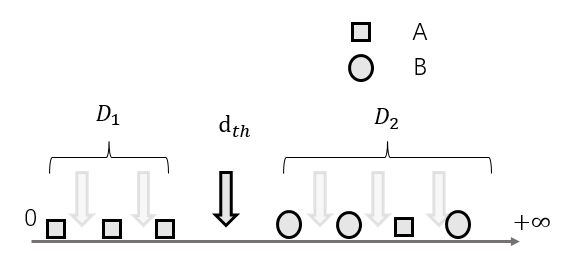
\includegraphics[height=4.2cm]{SubDistDistribution.png}
		\caption{$SubDist(S,T_j),T_j\in D$在$(0,\infty)$的分布}
		\label{fig:SubDist}
	\end{figure}
\end{definition}
	\begin{equation}
\label{equ:chap2:Infogain2}
g(D,(S,d_{th})) =H(D)-H(D|(S,d_{th})) = H(D)-(\frac{|D_1|}{|D|}H(D_1)+\frac{|D_2|}{|D|}H(D_2))
\end{equation}	
\begin{definition}
	\label{def:optimalsplitpoint}
	最佳分割点:在候选序列$S$下,有多个阈值$d_{th}$,如图~\ref{fig:SubDist},在这些分割点中,存在一个阈值$d_{osp(S)}$(或者是一段区间),满足$g(D,(S,d_{osp(S)})) \geq g(D,(S,d_{th})),\forall d_{th}\in \mathbb{R}_{+}$,则将$d_{osp(S)}$记为候选序列$S$对应的最佳分割点。
\end{definition}
数据集$D$中有$O(NL^2)$个候选序列,即有$O(NL^2)$个特征组合$(S,d_{osp(S)})$,需要选取分类能力最高的特征组合,分类能力最高特征组合中的候选序列即为Shapelet,如定义~\ref{def:choose}。
\begin{definition}
	\label{def:choose}
	数据集$D$中的Shapelet,使用$Shapelet(D)$表示。对于给定数据集,存在一个子序列$Shapelet(D)$,使$g(D,(Shapelet(D),d_{osp(Shapelet(D))})) \geq g(D,(S,d_{osp(S)})),\forall S\in SubSet(D)$。$(Shapelet(D),d_{osp(Shapelet(D))})$特征将作为Shapelet算法那最终的分类器。
\end{definition}
\begin{definition}
	\label{def:chap03:Threephases}
	Shapelet计算过程三阶段:本文将Shapelet计算过程分为三个阶段,分别为距离计算阶段、最佳分割点计算阶段、候选序列筛选阶段。其中距离计算阶段是指从候选序列$S$和数据集$D$到$S$相对数据集$D$所有时间序列计算距离获取距离-类标对的集合$\mathcal{F}$的过程,即计算$\mathcal{F}$的过程;最佳分割点计算阶段是指从$\mathcal{F}$到对应的最佳分割点$d_{osp(S)}$以及对应的信息增益的过程,相当于定义~\ref{def:optimalsplitpoint}过程;候选序列筛选阶段是指从多个候选序列中选出分类能力最高的候选序列,相当于定义~\ref{def:choose}过程。章节~\ref{cha:chap03:Problemsencountered:BigDataSet}解释了为什么从中间结果$\mathcal{F}$处分成两个阶段,章节~\ref{cha:chap03:modelduty}解释了为了要从最佳分割点处分为两个阶段。
\end{definition}

从以上定义来看,时间序列可以分类的前提是,数据集中的一类(比如$A$类)存在一种模式(波形),这种模式和$A$类时间序列($T_j,y_i\in A$)表现出较小的距离,和另一类$B$类时间序列($T_j,y_i\in B$)表现出较大的距离。而Shapelet算法那就是负责寻找能够区分这两类时间序列的模式以及对应的距离阈值的算法。%Shapelet对于所有的候选序列$(S,d_{osp(S)})$按照对于$D$的信息增益进行评价,选出信息增益最大的候选序列和对应的距离阈值$(Shapelet(D),d_{osp(Shapelet(D))})$。

\section{通用算法分析}
\label{cha:chap02:generalalganalysis}
\begin{algorithm}
	\caption{Shapelet原始算法}
	\label{alg:origin}
	\begin{algorithmic}[1]
		\Function{ShapeletNaiveAlg}{$D$}
		%\State $CENTER \gets (w+1)/2$;
			\State $lastS \gets \phi, lastinfogain \gets 0, lastdosp \gets 0, leftisAorB\gets A$ 
			\ForAll{$S \in SubSet(D)$} \label{Code:Set} //O($NL^2$)个候选序列
				\State $\mathcal{F} = \left\lbrace (...,SubDist(S,T_j),y_j),...\right\rbrace,j = 1,2,\cdots,N$ \label{Code:calcSubDist} //O($NL^2$)
				\State 计算$g(D,(S,d_{osp(S)}))$ \label{Code:infogain}  //O($N\log(N)$)
				\If{$g(D,(S,d_{osp(S)})) > lastinfogain$}
					\State 更新$lastinfogain$,$lastS$,$lastdospd_{osp(S)}$,$leftisAorB$
				\EndIf
			\EndFor
			\State \Return $lastinfogain,lastS,lastdops,leftisAorB$
		\EndFunction
	\end{algorithmic}
\end{algorithm}

如算法~\ref{alg:origin}为Shapelet发现的通用算法,是所有子序列中发现具有最佳分类能力的子序列的过程。其中:

$line$~\ref{Code:calcSubDist}是对于计算一个候选序列$S$相对于数据集$D$中每个时间序列$T_j$的过程,时间复杂度为$O(NL^2)$;

$line$~\ref{Code:infogain}是寻找一个阈值$d_{osp(S)}$与候选序列$S$共同作为特征满足$g(D,(S,d_{osp(S)})) \geq g(D,(S,d_{th})),\forall d_{th}\in \mathbb{R}_{+}$,时间复杂度为$O(N\log(N))$。

$line$~\ref{Code:Set}:$SubSet(D)$集合大小为$O(NL^2)$,因此$line$~\ref{Code:Set}处循环为$O(NL^2)$次;循环内部时间复杂度为$O(NL^2)$。

%对于数据集$D$中所有候选序列$SubSet(D)$都经过$line$~\ref{Code:calcSubDist}-\ref{Code:infogain}两步的评估过程,$SubSet(D)$集合大小为$O(NL^2)$。
因此Shapelet通用算法的时间复杂度为$O(N^2L^4)$,这个时间复杂度非常高,特别$N,L$比较大的情况,严重地影响执行时间。

\section{相似度/距离度量方法}
\label{cha:chap02:Distance}

章节~\ref{cha:chap02:def}描述的相似度/距离计算都是基于两个时间(子)序列$A,B$的相似性度量$Dist(A,B)$进行的,本章节就$Dist(A,B)$展开介绍。时间序列相似性/距离是许多计算系统的核心,同时也是时间序列聚类和分类的最重要的组成部分之一~\cite{patidar2012analysis}。正是由于相似度/距离度量的重要性,多种相似度/距离度量的方法先后被提出。在本章节中,我们对于几个具有代表性的时间序列相似度/距离度量及其所属类别进行评估,相似度/距离计算可以简单分为\cite{ding2008querying}:锁步距离测量(欧氏距离)、基于特征测量(傅里叶系数)、基于模型测量(自回归)、弹性测量(动态时间规整、实数序列的编辑距离)。

在上述多种相似性计算当中,基于特征测量和基于模型测量都没有直接利用时间序列之间的距离而是使用时间序列提取的特征进行计算相似性的,和Shapelet算法的滑动窗口距离取最小值的方法不符,因此对于这两种距离不予考虑。

对于两个时间序列$A=\left\lbrace a_1,a_2,\cdots,a_M\right\rbrace$和$B=\left\lbrace b_1,b_2,\cdots,b_M\right\rbrace$,本章主要讨论欧氏距离、实数序列的编辑距离、动态时间规整距离进行介绍并比较。

\subsection{欧氏距离}
欧氏距离是使用最普遍的距离度量方法,是度量$M$维空间上的两个点的直线距离,使用$Dist(A,B)$或者$Euclid(A,B)$表示。将欧氏距离应用在时间(子)序列上,要求两个时间序列$A,B$的长度相等$|A|=|B|$。在实际使用中经常将欧式距离的定义会进行扩展,使用两个长度相等时间序列$A,B$的差的$L_n$范数作为欧氏距离~\cite{serra2014empirical},如公式~\ref{equ:chap2:DistEuclid}。有时候,为了便于计算,经常使用$\sum_{i=1}^{M}(A_i-B_i)^n$记做欧氏距离,其中$n=1$,为曼哈顿距离,$n=2$,为狭义欧氏距离,$n$一般会作为一个底层距离参数,可以根据情况调节。
\begin{equation}
\label{equ:chap2:DistEuclid}
Euclid(A,B) = (\sum_{i=1}^{M}(A_i-B_i)^n)^{\frac{1}{n}}
\end{equation}

欧氏距离的优点在于计算简单,复杂度低;缺点要求两个时间序列各元素一一对应,不能弹性地计算时间序列之间距离,不能扭曲对应,这也是欧氏距离属于锁步距离的原因。

%对于长度都为$M$的两个时间(子)序列$A$和$B$,两者之间的欧氏距离是两者对应元素平方和的平方根,如~\ref{equ:chap2:DistEuclid}。为了简化计算,经常使用平方和$\sum_{i=1}^{M}(A_i-B_i)^2$表示$Dist(A,B)$。
%
%欧氏距离之所以称为锁步距离,就是需要元素一一对应

\subsection{动态时间规整}
\label{cha:chap02:dtw}


动态时间规整\cite{muller2007dynamic}(Dynamic Time Warping,~DTW)是一种通过将一个时间序列$A$延时间轴进行非线性的延展或者压缩,目的使$A$序列和另一时间序列$B$能够很好地对齐,对齐方式如图~\ref{fig:twoplotdtw}。这种对齐方式是可以通过一种动态规划的算法计算获得,如图~\ref{fig:threeplotdtw},图中从$(0,0)$到$(|A|,|B|)$的路线称为规整路径。

\begin{figure}
	\begin{minipage}{0.48\textwidth}
		\centering
		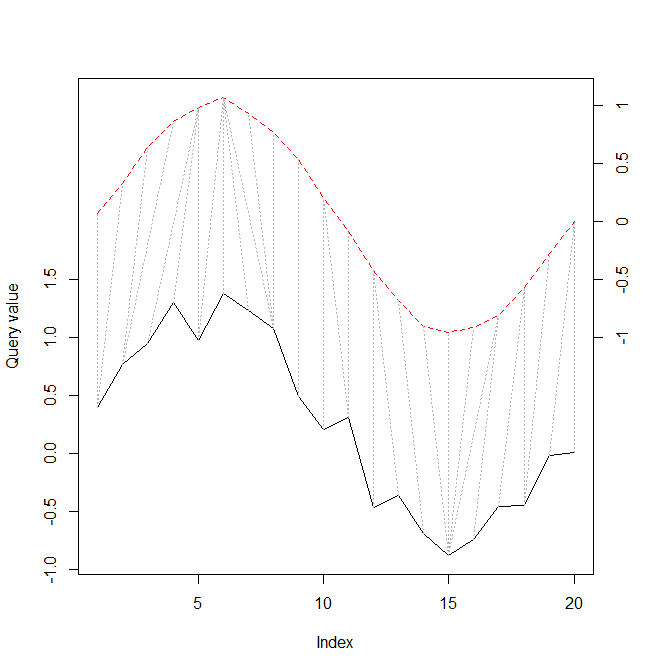
\includegraphics[height=6.2cm]{twoplotdtw.png}
		\caption{时间序列$A,B$对齐方式}
		\label{fig:twoplotdtw}
	\end{minipage}\hfill
	\begin{minipage}{0.48\textwidth}
		\centering
		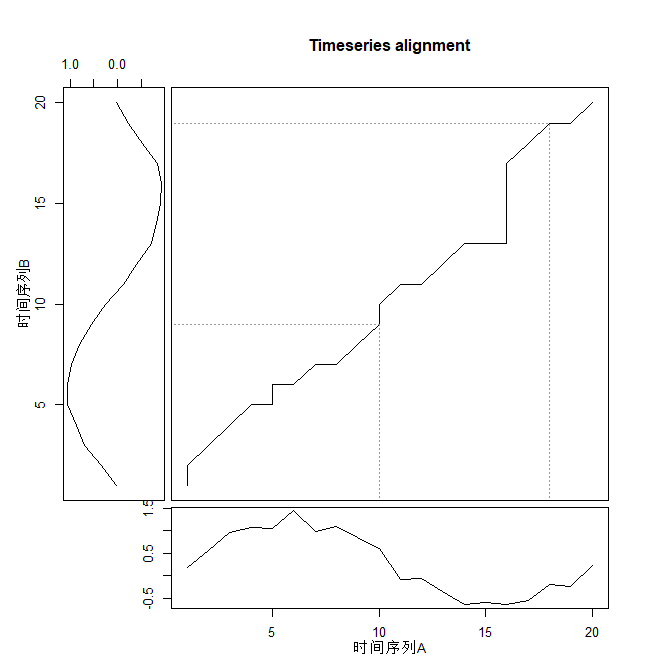
\includegraphics[width=6.2cm]{threeplotdtw.png}
		\caption{时间序列$A,B$规整路径和代价矩阵}
		\label{fig:threeplotdtw}
	\end{minipage}
\end{figure}

$A$和$B$之间的DTW距离用$DTW(A,B)$来表示,$DTW(A,B)$的递归方程如公式~\ref{equ:chap2:costMatrix}~\cite{sart2010accelerating}\footnote{n=1,2}。
\begin{equation}
\label{equ:chap2:costMatrix}
\begin{array}{l}
Dist(A,B) = d(M,M) \\ [0.3cm]
d(i,j) = |a_i-b_j|_n + \min
\begin{cases}
d(i-1,j)\\
d(i,j-1)\\
d(i-1,j-1)
\end{cases}\\[0.2cm]
d(0,0)=0;d(i,0)=\infty;d(0,j)=\infty;i=1,2,\cdots,M;j=1,2,\cdots,M 
\end{array}
\end{equation}


我们要求上面递推公式~\ref{equ:chap2:costMatrix}比较的两个时间序列长度是相等的$|A|=|B|= M$,但其实DTW不要求时间(子)序列长度一致。这里要求$|A|=|B|= M$主要基于两个原因考虑:第一,这样对于任何一个子序列$S$与$T_j$的距离,如果不要求(子)序列长度一致,就必须计算$T_j$所有子序列和$S$的DTW距离,然后在这些距离中取最低值,这样$S$需要和$O(L^2)$个子序列计算距离,使计算的复杂度变高;第二,不能判断哪个时间序列更具相似性,比如有$D,E,F$三个时间序列,其中$|D|<<|E|<|F|$,$DTW(D,E) < DTW(F,E)$,但是这里不能就此认定对于$E$,$D$比$F$更具有相似性。

递归方程~\ref{equ:chap2:costMatrix}计算DTW距离的时间复杂度和空间复杂度都是$O(M^2)$(如果$|A|=|B|=M$),相比于欧氏距离都很大。因为DTW时间空间复杂度高的原因,有人提出了FastDTW\cite{salvador2007toward},通过将规整路径限制在一定区域内来加速计算,限制区域主要包括$Sakoe-Chuba band$(如图~\ref{fig:Sakoe-Chuba-band})和$Itakura band$(如~\ref{fig:Itakura-band})两种方法。这两种限制区域的方式实质上将时间序列扭曲对应限制在一定的范围内。

本文使用到的是Sakoe-Chuba-band限制区域方法,这里需要对它进行介绍。如图~\ref{fig:Sakoe-Chuba-band},Sakoe-Chuba-band限制区域沿反对角线方向向两边延展,而$w$是一个控制限制区域宽度的参数,这里使用$DTW(A,B,w)$表示时间序列$A,B$之间的$w$参数下限制区域DTW距离。$w(w>=0)$作为限制区域的宽度的参数,当$w=0$时,限制区域为反对角线;当$w=M$(与时间序列$A,B$长度相等)时,限制区域为整个代价矩阵区域,这个时候限制区域DTW距离计算退化为于原始的DTW距离。因为$DTW(A,B)$或者$DTW(A,B,w=M)$距离是限制区域$DTW(A,B,w)$距离的特殊形式,后文提到的DTW距离都是指$DTW(A,B,w)$距离,而原始的DTW距离将会用$DTW(A,B,w=M)$来表示。

算法~\ref{alg:fastdtw}是$DTW(A,B,w$距离计算的算法,时间复杂度和空间复杂度都为$O(wM)$。

\begin{figure}
	\begin{minipage}{0.48\textwidth}
		\centering
		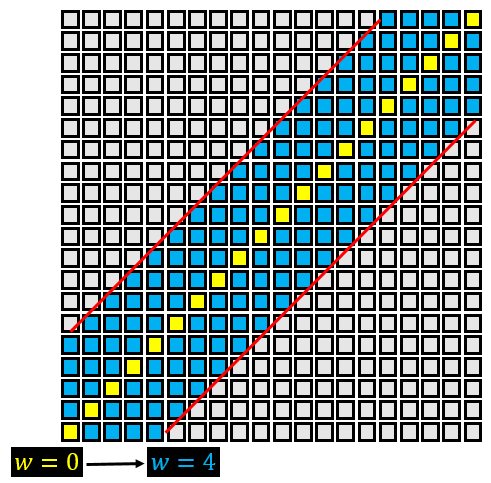
\includegraphics[height=6.2cm]{Sakoe-Chubaband.png}
		\caption{Sakoe-Chuba-band限制区域}
		\label{fig:Sakoe-Chuba-band}
	\end{minipage}\hfill
	\begin{minipage}{0.48\textwidth}
		\centering
		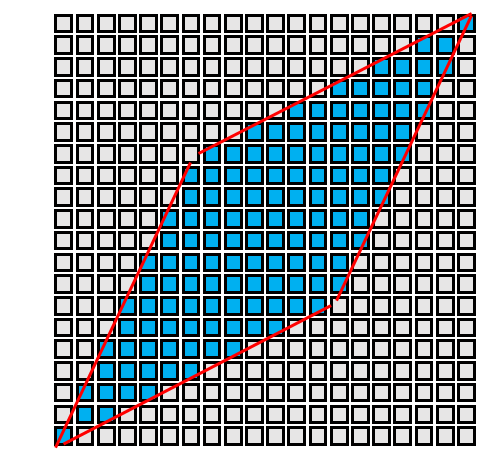
\includegraphics[width=6.3cm]{Itakuraband.png}
		\caption{Itakura-band限制区域}
		\label{fig:Itakura-band}
	\end{minipage}
\end{figure}

\begin{breakablealgorithm}
	\caption{DTW距离计算($Sakoe-Chuba-band$限制区域)}
	\label{alg:fastdtw}
	\begin{algorithmic}[1]
		\Function{DTW}{$A,B,w$}  //$|A|=|B|=M$
			\State $D = array(M+1,M+1)$
			\For{$m = 0$ to $M$}
				\If{$m < w$}
					\State $D_{m,0} \gets \infty, D_{0,m} \gets \infty$
				\Else
					\State $D_{m,w+m} \gets \infty, D_{w+m,m} \gets \infty$
				\EndIf
			\EndFor
			
			\For{$m = 1$ to $M$}
				\For{$n = \max(m-w,1)$ to $\min(M,m+w)$}
					\State $D_{m,n} = \min(D_{m-1,n-1},D_{m-1,n},D_{m,n-1}) + d(a_m,b_n)$
				\EndFor
			\EndFor
			\State \Return $D_{M,M}$
		\EndFunction
	\end{algorithmic}
\end{breakablealgorithm}

\subsection{实数序列的编辑距离}
实数序列的编辑距离~\cite{chen2005robust}(Edit Distance on Real Sequence,~EDR)可以视为原始编辑距离算法在实数序列领域的扩展,递归方程如公式~\ref{equ:chap2:EDR}。
\begin{equation}
\label{equ:chap2:EDR}
\begin{array}{l}
EDR(A,B) = d(M,M) \\ [0.3cm]
d(i,j) = \begin{cases}
i & \text{if }j=0 \\
j & \text{if } i=0 \\
d(i-1,j-1) & \text{if } \theta(a_i-b_j,\epsilon) \\
\min(d(i,j-1),d(i-1,j-1),d(i-1,j)) + 1 & \text{otherwise} \\
\end{cases}\\[0.2cm]
\end{array}
\end{equation}
EDR要求时间序列长度相等$|A|=|B|$,主要是基于和DTW距离相同的考虑。其中,$\theta$是一个阶跃函数,参数$\epsilon$,$\epsilon\in [0,\infty)$是一个控制两个序列样本$a_i,b_j$是否匹配的阈值参数,在实际的EDR计算中,$\epsilon$作为一个超参数需要提前确定。但是如果将EDR应用到Shapelet中,这样的参数$\epsilon$难以确定,对于某一个数据集适应的$\epsilon$不一定适应于其他数据集。

%,因为在Shapelet发现过程中,存在大量不同长度的候选序列$S_1,S_2,|S_1|\neq |S_2|$和分别和时间序列子序列$T_{j,s}^{|S_1|},T_{j,s}^{|S_2|}$进行距离计算,$EDR(S_1,T_{j,s}^{|S_1|})$和$EDR(S_2,T_{j,s}^{|S_2|})$的计算不能使用相同的$\epsilon$参数来度量距离。


\subsection{欧式距离与动态时间规整比较}
\label{chap02:euclid2Dtw}

%在过去的十年中,已经提出了超过一百种不同的时间序列距离测量方法[12]。 然而越来越多的经验证据表明动态时间翘曲(DTW)(包括欧几里得距离作为一种特殊情况)是跨越广泛领域的最佳测量方法[7]。
%[12]Keogh, E. J. and Kasetty, S. On the Need for Time Series Data Mining Benchmarks: A Survey and Empirical Demonstration. Data Min. Knowl. Discov. 7(4): 349-371 (2003).

如图~\ref{fig:Sakoe-Chuba-band},当$w=0$时,DTW代价矩阵将会退化成代价矩阵的对角线,$D(i,j)$的递推方程也将变为沿对角线递归,如图~\ref{fig:Sakoe-Chuba-band}黄色部分和~\ref{equ:chap2:dtwdeg2euclid1}递归方程,因此,当$w=0$时,时间序列的距离$DTW(A,B,0)$则退化欧式距离。

当$w=0$时,在DTW距离计算等价于欧氏距离,但是相比欧式距离会多出$2M$个比较计算过程和$2M$次访存过程。
\begin{equation}
\label{equ:chap2:dtwdeg2euclid1}
\begin{array}{l}
d(i,j) = |a_i-b_j|_n + \min
\begin{cases}
d(i-1,j)\\
d(i,j-1)\\
d(i-1,j-1)\\
\end{cases} = |a_i-b_j|_n + d(i-1,j-1)
\\[0.2cm]
d(0,0)=0 \\[0.2cm]
DTW(A,B,0) = d(M,M) = \sum_{i=1}^{M}|a_i-b_i|_n = Euclid(A,B)
\end{array}
\end{equation}



\subsection{相似度/距离度量方法选择}

在章节~\ref{cha:chap02:Distance}前面部分介绍各种相似度/距离以及存在的联系。本章节需要选出适用的相似度/距离计算作为Shapelet的相似度/距离调用子程序。

欧式距离$Euclid(A,B)$是Shapelet原始算法的相似度/距离度量,是时间序列数据挖掘应用上有很健壮的性能指标。欧式距离相比其他距离度量的优势在于时间复杂度低,但由于欧氏距离是锁步距离,要求序列上的元素一一对应。

DTW距离$DTW(A,B,w)$容许时间序列进行局部延长和压缩,能够克服欧氏距离由于时间序列发生扭曲而无法进行匹配的问题。DTW距离的时间复杂度为$O(wM)$,这里$w$作为控制时间序列扭曲程度一个参数,一般比较小(只有时间序列过度扭曲才需要很大的限制区域即$w$很大来包含时间序列之间的规整路径),因此,$DTW(A,B,w)$中$w$取值范围为$\left[ 0,C\right),s.t. C << M $,时间复杂度仍为线性。章节~\ref{chap02:euclid2Dtw}对于欧氏距离和DTW关系进行了介绍,欧式距离是DTW的特殊形式,存在$DTW(A,B,w)\leq DTW(A,B,w=0) = Euclid(A,B)$关系,使用$DTW(A,B,w)$作为相似度/距离调用在保持欧式距离的健壮性基础上,可以使时间序列进行一定扭曲来进行匹配。

EDR需要提前确定一个超参数$\epsilon$或者对于$EDR(A,B)$中$A,B$进行标准化,所以不适合作为Shapelet作为相似度/距离调用。

综上所述,本文选择$DTW(A,B,w),w\in \left[0,C\right),s.t. C << M$作为Shapelet的相似度/距离度量。当$w>0$时,距离计算阶段采用的距离度量是$DTW(A,B,w)$;而当$w=0$时,为了避免不必要的计算,距离计算阶段采用$DTW(A,B,w)$距离度量的等价方案$Euclid(A,B)$。因此,距离计算阶段会根据$w$的不同分为:w>0距离计算模块和w=0距离计算模块。


\section{GPU/CUDA并行原理及相关优化技术}
\label{cha:chap03:gpu-HW-Arch}

GPU/CUDA并行采用单指令多数据(Single Instruction Multiple Data,~SIMD)并行方式的。SIMD并行是将数据元素映射到并行处理线程交由相同的程序处理。本章节首先从GPU硬件架构和CUDA并行原理方面进行介绍并行技术,其中,GPU硬件结构部分介绍GPU的硬件结构组成构成并行的基础,CUDA并行原理部分来说明CUDA如何利用GPU硬件完成并行任务的。然后在GPU/CUDA并行原理的基础上介绍本文用到的CUDA优化技术。GPU加速并行并没有改变算法的时间复杂度,而是在CPU执行时间的基础上除以一个常数,这个常数由两个因素决定,一是GPU结构及流处理器簇个数和每个流处理器簇中流处理器个数,二是与优化技术和算法的结合以及算法本身的实现有关。硬件基础没有办法改变,更多的是依靠算法实现和优化技术,一个高效的优化算法相比一般的优化算法也会有很大的速度区别,比如归约中的$kernel7$相比$kernel1$在$4M$元素下加速倍数为21倍~\cite{harris2007optimizing}。章节~\ref{cha:chap02:coalesced}-章节~\ref{cha:chap02:bankconflict}详细地介绍了本文用到的CUDA优化技术,包括合并内存访问、隐藏延时、线程束分歧、存储体冲突等

本章节的图~\ref{fig:GPU-HW-Arch}和图~\ref{fig:nvidia-cuda-arch}全部根据文献~\cite{nickolls2009graphics}和文献~\cite{lippert2009nvidia}综合绘制。本章节介绍GPU/CUDA并行和CUDA相关技术都是以英伟达的图形处理器为例介绍的,对于其他加速设备以及并行技术没有覆盖。
\subsection{GPU硬件结构}
\label{cha:chap03:gpu-Hw}
图~\ref{fig:GPU-HW-Arch}介绍了GPU的典型硬件结构,GPU硬件包括了流处理器、流处理器簇、内存(全局、共享、常量等)几个关键部分。下面从这个几个关键部分开始介绍GPU硬件结构。

流处理器(Streaming Processor,SP)是GPU最基本的单元( 计算单元),也是执行一个线程的基本单元,因此SP又称为CUDA核,如图~\ref{fig:GPU-HW-Arch}的SP。

流处理器簇(Stream Multiprocessors,SM)是由一定数量的SP加上指令单元、寄存器、共享内存、L1/L2缓存等组成。从图~\ref{fig:GPU-HW-Arch}可以看出,每个SM是一个SIMD处理单元,由多个SP和一个指令单元组成。而GPU实际上是一个SM的阵列,而SM又是由多个SP组成,GPU进行并行计算的本质就是众多SP共同进行数据计算的过程。以GTX-1080来讲,GPU含有20个SM,每个SM含有128个SP,即在GPU最多可以同时运行$20*128$个线程。
\begin{figure}[H] % use float package if you want it here
	\centering
	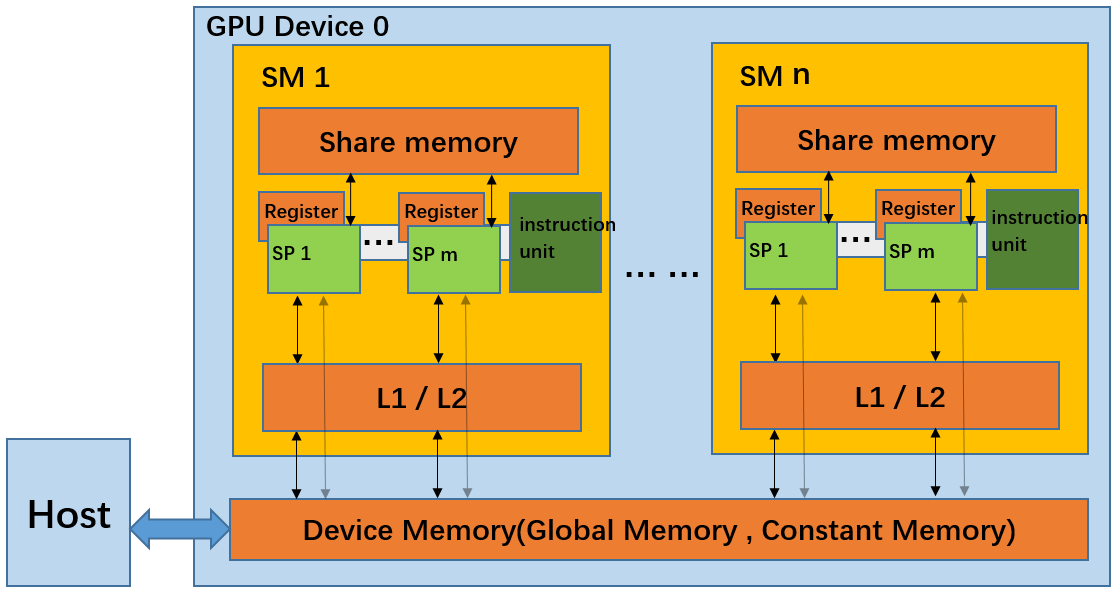
\includegraphics[height=7.2cm]{gpuarch.png}
	\caption{GPU硬件结构}
	\label{fig:GPU-HW-Arch}
\end{figure}

全局内存(Global  memory)是独立于GPU内核的内存,同时也是GPU中空间最大的内存,但访问延时最长,如图~\ref{fig:GPU-HW-Arch}。全局内存有以下特点:对于所有SP可见( 所有SP都可以读写全局内存);可以通过和主存建立主机和GPU之间的数据通信;两个并行任务之间的中间结果必须使用全局内存来处理。

共享内存(Share memory),是存在SM内部可以由SM内部多个线程共享使用的内存,速度是全局内存的几百倍。可以通过共享内存完成线程之间的通信和协作计算。共享内存对于某些特定的线程可见,具体后文会提及。

寄存器(Registers)是GPU中最快的内存,用于存储线程中的临时变量,只在线程内部可见。

本地内存(Local memory)是存储堆栈中无法容纳的所有内容的临时变量,本地内存存储在全局内存中,但对于线程可见。
\begin{table}[htbp]
	\centering
	\begin{minipage}{0.9\textwidth}
		\caption{GPU中各种存储之间的比较}
		\label{tab:memory}
		\begin{tabular}{p{2cm}p{2.1cm}p{3cm}p{2cm}p{2cm}}
			\toprule[1.5pt]
			{\heiti 内存种类} & {\heiti 访存延时} (时钟周期)&{\heiti 内存大小} &{\heiti 可见范围} &{\heiti 周期}\\\midrule[1pt]
			全局内存  & $\sim$400-600 & 8G  & 线程网格  & 整个过程 \\
			共享内存 & $\sim$20 & 48K(每个线程块) & 线程块 & 线程 \\
			寄存器 & $\sim$1 & 64K(每个线程块) & 线程块 & 线程 \\
			本地内存 & $\sim$400-600 & 同全局内存 & 线程块 & 线程 \\
			\bottomrule[1.5pt]
		\end{tabular}
	\end{minipage}
\end{table}

常量内存和纹理内存在本文中没有涉及,在这里不做介绍。

表~\ref{tab:memory}对于使用到的内存的性能进行比较,更好地理解各内存在程序中所起的功能。

\subsection{CUDA并行原理}

前面从硬件角度介绍GPU的硬件结构,本章节将从软件角度叙述CUDA如何在GPU的硬件基础进行并行计算的,首先介绍几个CUDA的基本概念。

线程(Thread)是并行程序的基本单元,一个并行程序是由很多线程共同执行,图~\ref{fig:nvidia-cuda-arch}带箭头的曲线表示一个线程。

线程块(Block)由多个线程组成,在一个Block中线程可以进行同步( 需要通过程序控制),也可以通过共享内存进行通信。如图~\ref{fig:nvidia-cuda-arch},每个$Block(x,y)$也是有线程的阵列组成,如$Block(1,1)$。

线程束(Warp),将Block连续线程ID聚合起来的32个线程(比如thread 0-31,32-63)定义为一个Warp,Warp是调度和运行的基本单元,Warp中所有线程并行的执行相同的指令并且是严格同步的,这种同步是由硬件底层完成而不需要通过程序来控制。Block会将连续的32个线程聚合成一个Warp,当一个Block的线程个数不是32个整数倍时,硬件会帮助不足32个线程的部分凑足32个线程形成一个Warp。

%因为SM是一个SIMD处理器,要求所有线程执行相同的指令,如果遇到分支语句,将会将两个分支串行执行。
线程网格(Grid),多个Block构成线程网格,Grid是主机程序调度的接口。如图~\ref{fig:nvidia-cuda-arch}所示,主机调用了两个Grid程序,其中Grid 1是由2*3个Block组成。

\begin{figure}[H] % use float package if you want it here
	\centering
	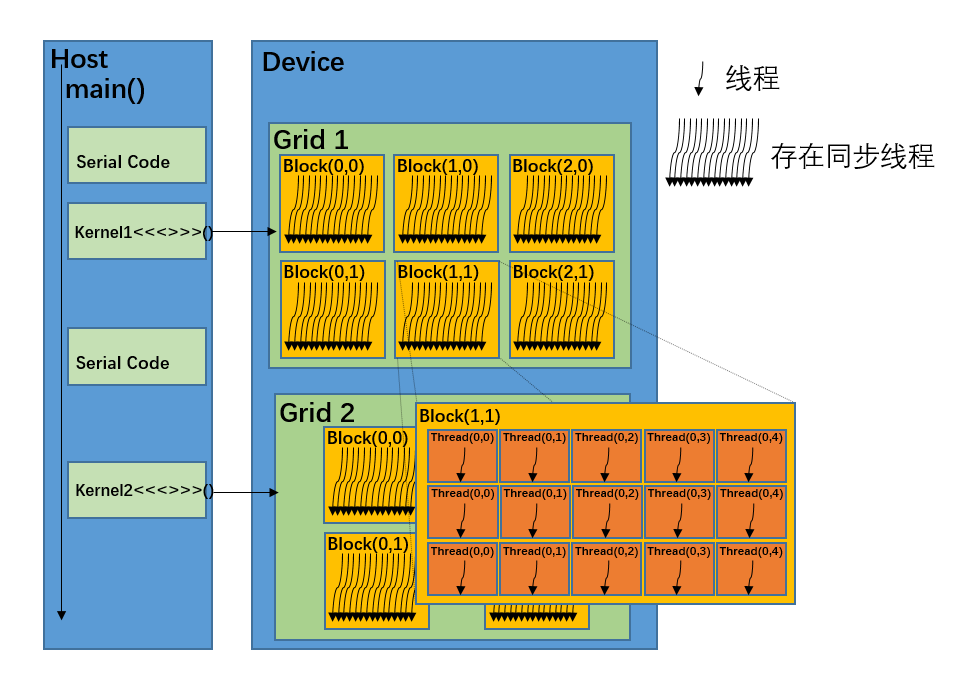
\includegraphics[height=7.5cm]{kernelexcute.png}
	\caption{NVIDIA CUDA架构}
	\label{fig:nvidia-cuda-arch}
\end{figure}

以GTX 1080为例,一个Grid最多可以有$2^{31}-1$个Block,一个Block最多可以有1024个线程,但是在硬件上每个GPU只有20个SM,每个SM只有128个。正常情况下2560个SP是不可能运行这么多线程的。

一个SP只能可以执行一个线程,但是实际上并不是所有的线程能够在同一时刻执行,SM运行线程也是采用了分时复用的思想。连续的32个线程形成一个Warp,一个Block中的1024个线程分成32个Warp。而GTX 1080一个SM有4个Warp调度单元,可以同时容纳4个Warp运行。起初所有Warp都在就绪队列中,首先从就绪对列取出4个Warp在SM上执行;当某个Warp因为读取内存操作或者其他原因而挂起时,Warp调度单元从就绪队列取出一个Warp执行;当正在内存请求的Warp完成内存请求之后,线程束将会进入就绪状态;当线程束执行完任务时进入结束状态;这样不断循环完成一个SM内所有Warp的执行。

多个Warp在4个Warp调度单元通过分时复用的方式进行并行运行,同样道理,一个Grid中大量的Block在20个SM中运行的原理是一致的,都是利用计算资源分时复用的方法。CUDA并行是由成千上万的线程并行完成的,这些线程在软件层面是同时并行的,但是在物理层面最多只有2560个线程在运行,其他都在挂起或者就绪状态。

\subsection{合并内存访问}
\label{cha:chap02:coalesced}

从表~\ref{tab:memory}可以看出访问全局内存是内存访问耗时最长的环节,但全局内存又是GPU内存最大的部分,当处理大量数据的并行时,不可避免地使用全局内存,这样必然导致大量的全局内存读写操作而产生访存延时,全局内存访问有可能成为性能优化的瓶颈。这里可以通过合并内存访问~\cite{nvidia2012c}来解决全局内存访问耗时问题。

合并内存访问(Coalesced Memory Access,~Coalesced),是当特定的访问条件满足时,设备可以将一个Warp内所有线程的全局内存访问操作合并成一个事务。这里特定的条件是一个Warp内线程访问连续的128B空间,而且线程和全局内存地址一一对应( 但不要求严格顺序对齐),如图~\ref{fig:coalesced}~\cite{woolley2013gpu}。这种合并内存访问模式只需要经过一次L1缓存的过程,大大地提高了全局内存访问速度,由图~\ref{fig:coalesced}红色区域表示。

\begin{figure}[H] % use float package if you want it here
	\centering
	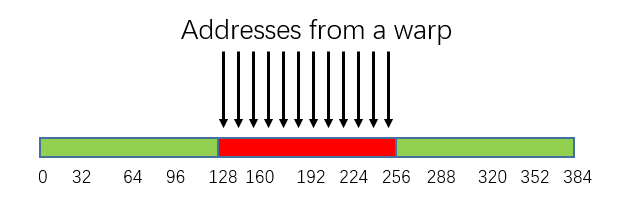
\includegraphics[height=2.5cm]{coaleced.png}
	\caption{合并内存访问(所有线程一个L1缓存行)}
	\label{fig:coalesced}
\end{figure}
合并内存访问加速全局内存访问可以通过Cache命中观点来解释:当一个Warp的32线程同时读写连续的128B空间,假设某个线程首先读取了128B空间中的某个地址,设备会将这连续的128B空间缓存到L1缓存行中(设备中L1缓存行的大小为128B),其他31个线程再进行读写这个128B地址空间时,可以直接命中到L1缓存行,而Cache的访问时延远小于全局内存,不需要经过内存读写挂起的过程,大大地降低了访问时延。

当一个warp的连续线程访问连续空间但没有按照L1对齐时,会请求两个128B的L1缓存行,如图~\ref{fig:Nocoaleced},会出现两次缓存L1的过程,至少需要经过两个全局内存时延等待。而且这种情况一般会伴随着同一个128B地址被两个warp访问,如果同一个128B地址被两个warp访问,而且这两个warp又不在一个SM中,就会因为考虑数据一致性的问题而导致延时。

\begin{figure}[H] % use float package if you want it here
	\centering
	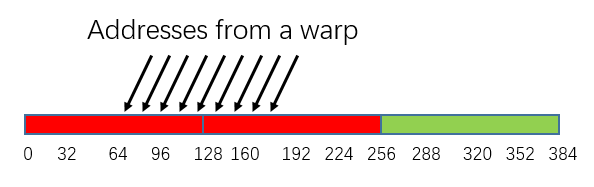
\includegraphics[height=2.5cm]{Nocoaleced.png}
	\caption{非对齐顺序地址访问(使用两个128B)}
	\label{fig:Nocoaleced}
\end{figure}

合并内存访问大大减少了全局内存访问时延,一般数据量过大的并行计算都是需要全局内存配合合并内存访问来解决。同时,合并内存访问、全局内存、共享内存结合使用可以完成很多复杂操作,比如矩阵转置等。

%为了尽量减少全局内存访问延时,减少等待时间,一方面需要增加一个Block内的Warp个数,对于访存时间进行隐藏,另外一方面,使用合并内存访问减少全局内存访问时延出现的次数。%将一个warp内多个线程计算的结果存储在连续的全局内存地址上,并且保证一个Warp对应能够缓存的128B地址。

\subsection{延时隐藏}

线程不可避免会出现访问各种内存访问而产生的访存延时,为了使访存延时不影响执行速度,可以使用隐藏延时的方法来解决。SM使通过调度Warp来执行线程,可以通过增加Warp的个数来使Warp调度单元尽可能选择已经就绪的Warp,避免选择正在因为延时而挂起的Warp。将通过执行多个Warp来获取较高吞吐量的方法称为隐藏延时。

对于这种性能度量通常通过占用率来评价,占用率通过并行执行的Warp数量除以并发运行的最大可能Warp数量。高占用率意味着Warp调度器有很多Warp可供选择,能够隐藏延时访存等。

在实际优化中,可以对于一个Block中执行的Warp个数进行调节,选择执行时间最短的。另外尽量避免全局内存访存之后出现同步操作,这样容易使访存时间没有办法隐藏。
%如果存在访存等延时尽可能选择较多的warp.
%{\color{red}{按照下面方法计算占有率,这个得做实验}}
%较高的占用率并不总是等同于较高的性能 - 有一点超出额外占用率不会提高性能。 但是,低占用率总是会干扰隐藏内存延迟的能力,从而导致性能下降。在于评价?
%http://docs.nvidia.com/cuda/cuda-c-best-practices-guide/index.html#memory-optimizations    Execution Configuration Optimizations
%尽量增加SM上的线程数量,提高Occupancy(实际并发运行的warp个数/最大可能并发运行的warp个数);
%http://blog.163.com/wujiaxing009@126/blog/static/71988399201709105252458/
%a. 限制条件:# of registers和# of shared memory, 一个SM可以并行处理768 threads
%b. 100%Occupancy: 2 blocks X 384 threads
%3 blocks X 256 threads
%4 blocks X 192 threads
%6 blocks X 128 threads
%8 blocks X 96 threads
%c. 最小存储器延时:Occupancy≥50% and threads/blocks≥128
%(2) Thread block内的线程个数应该是warp size的整数倍,避免在一个warp内有分支语句;
%(3) Grid/Block Size Heuristics;
%a. # of blocks / # of SMs > 1
%每个SM至少有一个thread block可以执行
%b. 更好的选择:# of blocks / # of SMs > 2
%每个SM有多个thread block可以执行
%c. 每个block占用SM一半以下的资源
%d. # of blocks > 100 使得适应将来的结构
%线程指令是在CUDA中顺序执行的,因此,当一个warp暂停或停顿时执行其他warp是隐藏延迟和保持硬件繁忙的唯一方法。 因此,在确定硬件保持繁忙的有效程度时,与多处理器上的活动warp数相关的一些度量标准非常重要。 这个度量是占用率

\subsection{线程束Warp分歧}

因为线程束Warp使GPU调度得基本单元,每个SM又是SIMD处理器(只有一个指令单元,但有多个处理器),因此Warp内的线程只能执行同一条指令。当遇到分支语句时,不同的线程需要执行不同的语句,这和Warp内线程只能执行一个指令互相矛盾。为了解决这个矛盾,分支语句会被序列化,一个Warp中同时只能执行一个分支即部分线程执行,其他分支的线程都处于挂起状态,这样会导致性能的降低,这种现象称为线程束分歧(Warp divergence,Warp分歧)。

为了Warp分歧影响GPU并行效率,尽量避免同一个Warp存在不同的分支路径,如果不能避免Warp分歧的出现,则尽量保证Warp内少数线程执行的分支内容尽可能少,或者提前并行计算。

\subsection{共享内存使用和存储体冲突}
\label{cha:chap02:bankconflict}

前面提到共享内存,相比全局内存拥有更小的时延和更高的带宽,并且线程之间可以通过共享内存进行通信和协作计算,但是使用共享内存有一个前提条件:不能出现存储体冲突。

首先看一下SM中共享内存结构,一个SM上的共享内存实际上是被分为可以同时访问的同等大小的内存块(Bank),因此可以达到共享通信和增加带宽的作用。共享内存中的地址以4bytes为单位依次分配到16个存储体(Bank)中,如图~\ref{fig:bank},$\_\_share\_\_\quad int\quad data[128]$,假设,那么$data[0],data[16],\cdots$属于Bank0,$data[1],data[17],\cdots$属于Bank1,...。

当每个线程(半个Warp)访问不同Bank时,可以快速读写共享内存,如图~\ref{fig:NobankConflict}。但当出现多个线程(半个Warp内)同时访问一个Bank的不同地址时,就会出现存储体冲突(Bank Conflict),这多个线程的访问将被序列化,分先后访问存储体(这部分工作是由硬件完成的),会造成多倍的访问时延,如图~\ref{fig:bankConflict},每个存储体被两个线程访问称为2-way Bank Conflict。但是有一个特殊情况,当一个Warp内的所有线程访问一个存储体中的同一个地址时,共享内存会将这个地址下的数据广播到Warp所有线程中,本文没有涉及,不作详述。

\begin{figure}
	\begin{minipage}{0.3\textwidth}
		\centering
		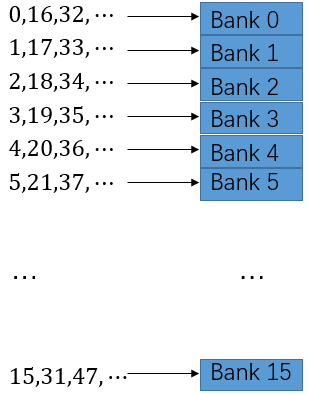
\includegraphics[height=5.5cm]{bank.png}
		\caption{共享内存存储体}
		\label{fig:bank}
	\end{minipage}
	\hfill
	\begin{minipage}{0.30\textwidth}
		\centering
		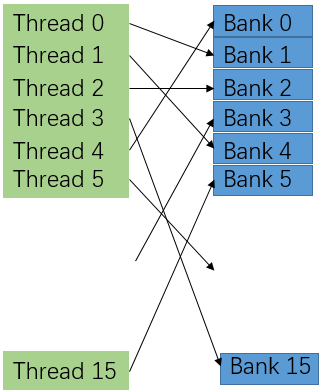
\includegraphics[height=5.5cm]{banknoconflict.png}
		\caption{No bank Conflict}
		\label{fig:NobankConflict}
	\end{minipage}
	\hfill
	\begin{minipage}{0.30\textwidth}
		\centering
		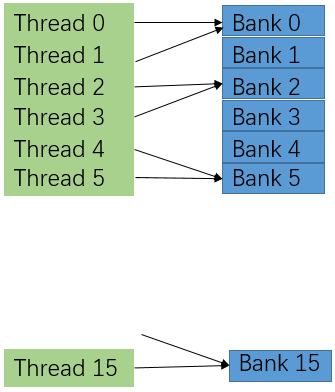
\includegraphics[height=5.5cm]{bankconflict.png}
		\caption{bank Conflict}
		\label{fig:bankConflict}
	\end{minipage}
\end{figure}

Bank Conflict经常出现在多个线程访问不连续的共享内存的情况下,当线程之间访问的共享内存间隔(Stride,4Bytes计为一个间隔)为固定的某个数比如2时,则每两个线程(thread0和thread9,thread1和thread10...)就会访问同一个存储体Bank,这样就会产生存储体冲突(Bank Conflict)。为了避免出现存储体冲突(Bank Conflict)现象,可以通过以下方法避免:

1.最好确保一个Warp的线程访问连续的一块共享内存,线程就能够访问到不同的存储体中;

2.使连续线程访问不连续共享内存地址,可以对其进行调整,比如访问矩阵的列,可以对矩阵先进行转置;

3.使用数据对齐的方式,尽量使用$int,float$占据4Bytes的格式,避免使用$double$等数据格式;

4.当线程不能访问连续的地址,而且访问的地址之间存在一个stride,需要保证stride=1,3,5,7,9...等奇数。


\section{本章小结}
%本章主要对于本文的基础算法和涉及到的GPU/CUDA加速技术进行了介绍。首先介绍Shapelet算法的相关定义和通用算法,并对通用算法时间复杂度进行了分析。然后对于不同的相似度度量方法进行了分析和比较,最后,详细介绍了GPU/CUDA并行原理以及本文并行工作使用到的CUDA优化技术。

本章首先介绍了Shapelet的相关定义和计算过程,为本文展开工作铺垫基础。然后对于Shapelet通用算法进行了描述,并分析了其时间复杂度,指明了Shapelet发现过程耗时的原因。然后对不同的相似度/距离度量方法进行了比较和分析,并对部分相似度/距离度量之间关系进行了介绍,选择了$DTW(A,B,w)$作为本文Shapelet方案的度量距离。最后对于GPU/CUDA并行原理和后文使用到的CUDA优化技术进行了详细介绍,为后文并行工作的描述打下基础。





%%% 其它部分
\backmatter

%% 本科生要这几个索引,研究生不要。选择性留下。
% 插图索引
\listoffigures
% 表格索引
\listoftables
% 公式索引
\listofequations


%% 参考文献
% 注意:至少需要引用一篇参考文献,否则下面两行可能引起编译错误。
% 如果不需要参考文献,请将下面两行删除或注释掉。
% 数字式引用
\bibliographystyle{thuthesis-numeric}
% 作者-年份式引用
% \bibliographystyle{thuthesis-author-year}
\bibliography{ref/refs}


%% 致谢
% 如果使用声明扫描页,将可选参数指定为扫描后的 PDF 文件名,例如:
% \begin{acknowledgement}[scan-statement.pdf]
\begin{acknowledgement}
  衷心感谢导师 xxx 教授和物理系 xxx 副教授对本人的精心指导。他们的言传身教将使
  我终生受益。

  在美国麻省理工学院化学系进行九个月的合作研究期间,承蒙 xxx 教授热心指导与帮助,不
  胜感激。感谢 xx 实验室主任 xx 教授,以及实验室全体老师和同学们的热情帮助和支
  持!本课题承蒙国家自然科学基金资助,特此致谢。

  感谢 \LaTeX 和 \thuthesis\cite{thuthesis},帮我节省了不少时间。
\end{acknowledgement}


%% 附录
\begin{appendix}
\chapter{外文资料原文}
\label{cha:engorg}

\title{The title of the English paper}

\textbf{Abstract:} As one of the most widely used techniques in operations
research, \emph{ mathematical programming} is defined as a means of maximizing a
quantity known as \emph{bjective function}, subject to a set of constraints
represented by equations and inequalities. Some known subtopics of mathematical
programming are linear programming, nonlinear programming, multiobjective
programming, goal programming, dynamic programming, and multilevel
programming$^{[1]}$.

It is impossible to cover in a single chapter every concept of mathematical
programming. This chapter introduces only the basic concepts and techniques of
mathematical programming such that readers gain an understanding of them
throughout the book$^{[2,3]}$.


\section{Single-Objective Programming}
The general form of single-objective programming (SOP) is written
as follows,
\begin{equation}\tag*{(123)} % 如果附录中的公式不想让它出现在公式索引中,那就请
                             % 用 \tag*{xxxx}
\left\{\begin{array}{l}
\max \,\,f(x)\\[0.1 cm]
\mbox{subject to:} \\ [0.1 cm]
\qquad g_j(x)\le 0,\quad j=1,2,\cdots,p
\end{array}\right.
\end{equation}
which maximizes a real-valued function $f$ of
$x=(x_1,x_2,\cdots,x_n)$ subject to a set of constraints.

\newtheorem{mpdef}{Definition}[chapter]
\begin{mpdef}
In SOP, we call $x$ a decision vector, and
$x_1,x_2,\cdots,x_n$ decision variables. The function
$f$ is called the objective function. The set
\begin{equation}\tag*{(456)} % 这里同理,其它不再一一指定。
S=\left\{x\in\Re^n\bigm|g_j(x)\le 0,\,j=1,2,\cdots,p\right\}
\end{equation}
is called the feasible set. An element $x$ in $S$ is called a
feasible solution.
\end{mpdef}

\newtheorem{mpdefop}[mpdef]{Definition}
\begin{mpdefop}
A feasible solution $x^*$ is called the optimal
solution of SOP if and only if
\begin{equation}
f(x^*)\ge f(x)
\end{equation}
for any feasible solution $x$.
\end{mpdefop}

One of the outstanding contributions to mathematical programming was known as
the Kuhn-Tucker conditions\ref{eq:ktc}. In order to introduce them, let us give
some definitions. An inequality constraint $g_j(x)\le 0$ is said to be active at
a point $x^*$ if $g_j(x^*)=0$. A point $x^*$ satisfying $g_j(x^*)\le 0$ is said
to be regular if the gradient vectors $\nabla g_j(x)$ of all active constraints
are linearly independent.

Let $x^*$ be a regular point of the constraints of SOP and assume that all the
functions $f(x)$ and $g_j(x),j=1,2,\cdots,p$ are differentiable. If $x^*$ is a
local optimal solution, then there exist Lagrange multipliers
$\lambda_j,j=1,2,\cdots,p$ such that the following Kuhn-Tucker conditions hold,
\begin{equation}
\label{eq:ktc}
\left\{\begin{array}{l}
    \nabla f(x^*)-\sum\limits_{j=1}^p\lambda_j\nabla g_j(x^*)=0\\[0.3cm]
    \lambda_jg_j(x^*)=0,\quad j=1,2,\cdots,p\\[0.2cm]
    \lambda_j\ge 0,\quad j=1,2,\cdots,p.
\end{array}\right.
\end{equation}
If all the functions $f(x)$ and $g_j(x),j=1,2,\cdots,p$ are convex and
differentiable, and the point $x^*$ satisfies the Kuhn-Tucker conditions
(\ref{eq:ktc}), then it has been proved that the point $x^*$ is a global optimal
solution of SOP.

\subsection{Linear Programming}
\label{sec:lp}

If the functions $f(x),g_j(x),j=1,2,\cdots,p$ are all linear, then SOP is called
a {\em linear programming}.

The feasible set of linear is always convex. A point $x$ is called an extreme
point of convex set $S$ if $x\in S$ and $x$ cannot be expressed as a convex
combination of two points in $S$. It has been shown that the optimal solution to
linear programming corresponds to an extreme point of its feasible set provided
that the feasible set $S$ is bounded. This fact is the basis of the {\em simplex
  algorithm} which was developed by Dantzig as a very efficient method for
solving linear programming.
\begin{table}[ht]
\centering
  \centering
  \caption*{Table~1\hskip1em This is an example for manually numbered table, which
    would not appear in the list of tables}
  \label{tab:badtabular2}
  \begin{tabular}[c]{|m{1.5cm}|c|c|c|c|c|c|}\hline
    \multicolumn{2}{|c|}{Network Topology} & \# of nodes &
    \multicolumn{3}{c|}{\# of clients} & Server \\\hline
    GT-ITM & Waxman Transit-Stub & 600 &
    \multirow{2}{2em}{2\%}&
    \multirow{2}{2em}{10\%}&
    \multirow{2}{2em}{50\%}&
    \multirow{2}{1.2in}{Max. Connectivity}\\\cline{1-3}
    \multicolumn{2}{|c|}{Inet-2.1} & 6000 & & & &\\\hline
    \multirow{2}{1.5cm}{Xue} & Rui  & Ni &\multicolumn{4}{c|}{\multirow{2}*{\thuthesis}}\\\cline{2-3}
    & \multicolumn{2}{c|}{ABCDEF} &\multicolumn{4}{c|}{} \\\hline
\end{tabular}
\end{table}

Roughly speaking, the simplex algorithm examines only the extreme points of the
feasible set, rather than all feasible points. At first, the simplex algorithm
selects an extreme point as the initial point. The successive extreme point is
selected so as to improve the objective function value. The procedure is
repeated until no improvement in objective function value can be made. The last
extreme point is the optimal solution.

\subsection{Nonlinear Programming}

If at least one of the functions $f(x),g_j(x),j=1,2,\cdots,p$ is nonlinear, then
SOP is called a {\em nonlinear programming}.

A large number of classical optimization methods have been developed to treat
special-structural nonlinear programming based on the mathematical theory
concerned with analyzing the structure of problems.
\begin{figure}[h]
  \centering
  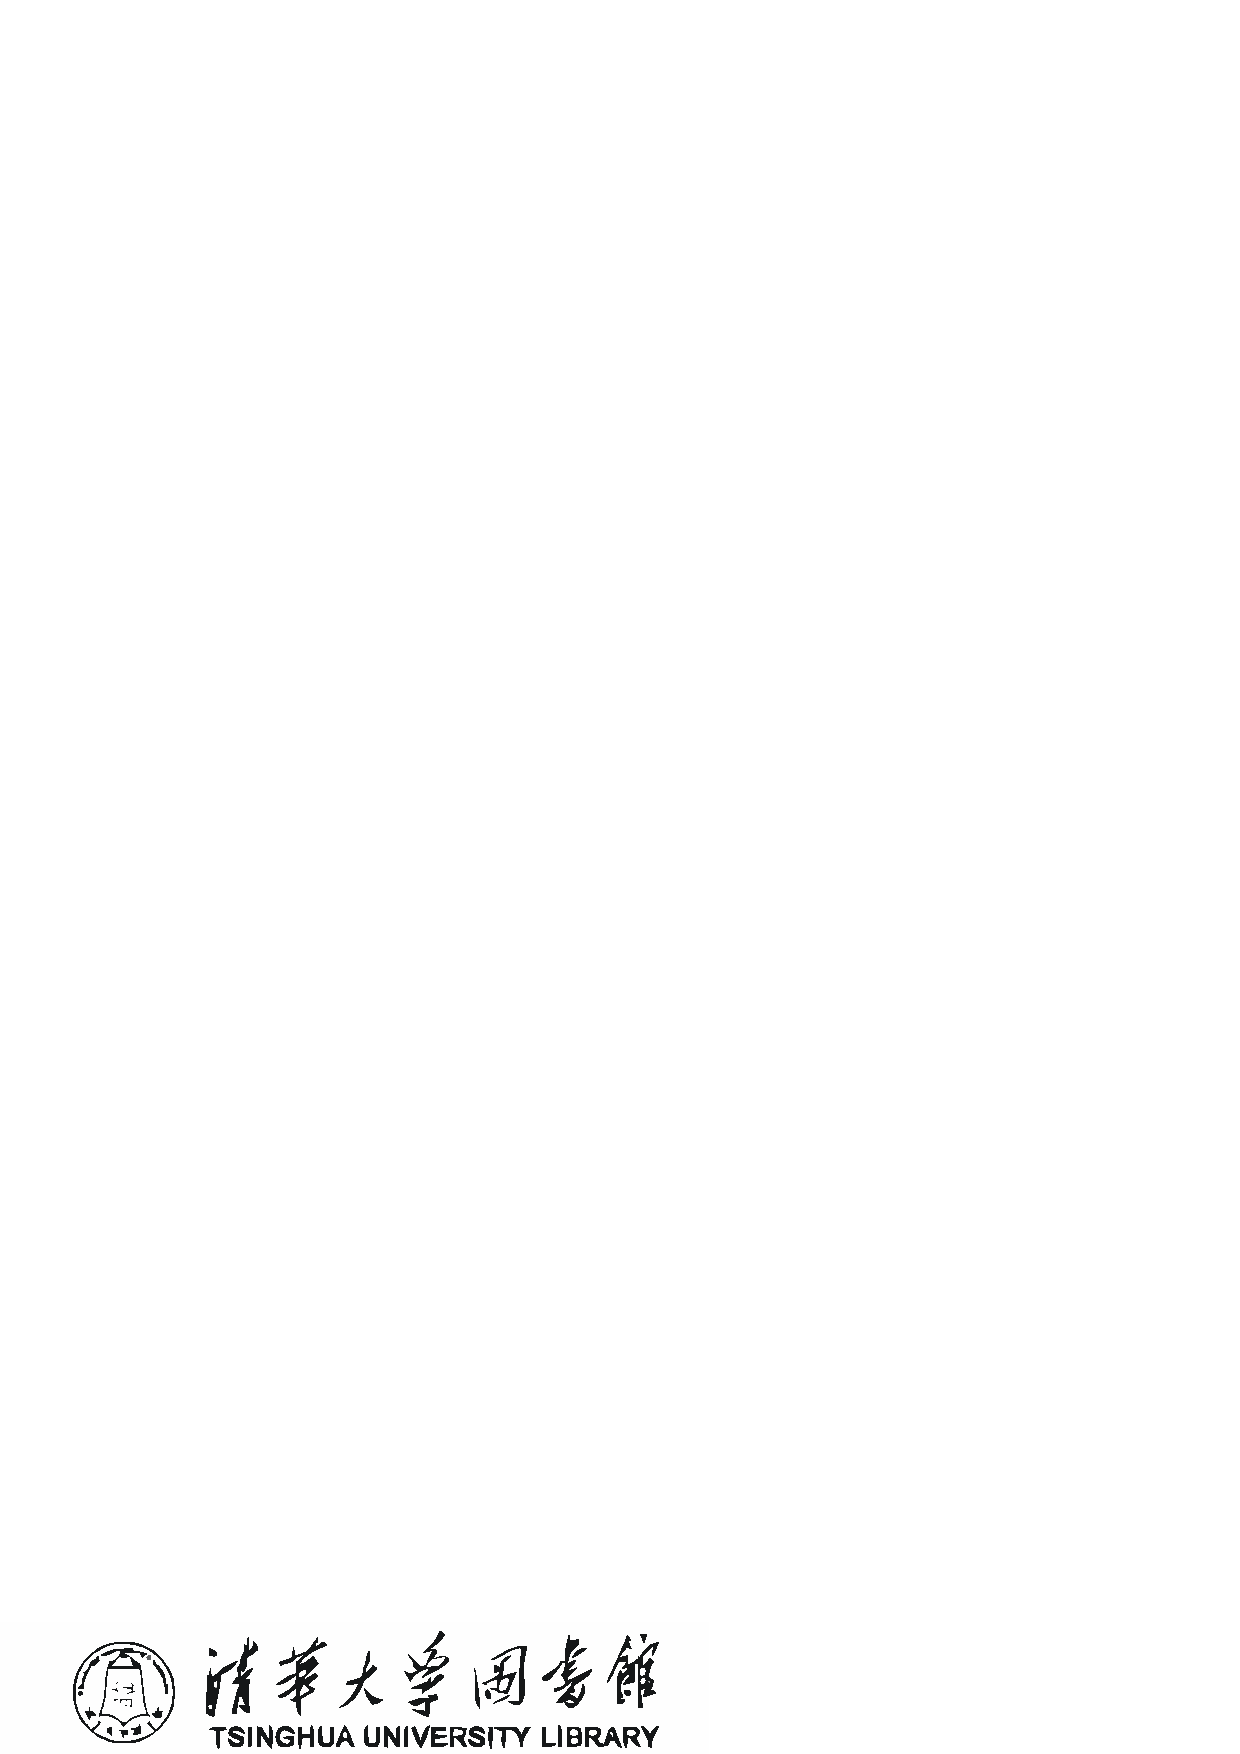
\includegraphics{thu-lib-logo}
  \caption*{Figure~1\quad This is an example for manually numbered figure,
    which would not appear in the list of figures}
  \label{tab:badfigure2}
\end{figure}

Now we consider a nonlinear programming which is confronted solely with
maximizing a real-valued function with domain $\Re^n$.  Whether derivatives are
available or not, the usual strategy is first to select a point in $\Re^n$ which
is thought to be the most likely place where the maximum exists. If there is no
information available on which to base such a selection, a point is chosen at
random. From this first point an attempt is made to construct a sequence of
points, each of which yields an improved objective function value over its
predecessor. The next point to be added to the sequence is chosen by analyzing
the behavior of the function at the previous points. This construction continues
until some termination criterion is met. Methods based upon this strategy are
called {\em ascent methods}, which can be classified as {\em direct methods},
{\em gradient methods}, and {\em Hessian methods} according to the information
about the behavior of objective function $f$. Direct methods require only that
the function can be evaluated at each point. Gradient methods require the
evaluation of first derivatives of $f$. Hessian methods require the evaluation
of second derivatives. In fact, there is no superior method for all
problems. The efficiency of a method is very much dependent upon the objective
function.

\subsection{Integer Programming}

{\em Integer programming} is a special mathematical programming in which all of
the variables are assumed to be only integer values. When there are not only
integer variables but also conventional continuous variables, we call it {\em
  mixed integer programming}. If all the variables are assumed either 0 or 1,
then the problem is termed a {\em zero-one programming}. Although integer
programming can be solved by an {\em exhaustive enumeration} theoretically, it
is impractical to solve realistically sized integer programming problems. The
most successful algorithm so far found to solve integer programming is called
the {\em branch-and-bound enumeration} developed by Balas (1965) and Dakin
(1965). The other technique to integer programming is the {\em cutting plane
  method} developed by Gomory (1959).

\hfill\textit{Uncertain Programming\/}\quad(\textsl{BaoDing Liu, 2006.2})

\section*{References}
\noindent{\itshape NOTE: These references are only for demonstration. They are
  not real citations in the original text.}

\begin{translationbib}
\item Donald E. Knuth. The \TeX book. Addison-Wesley, 1984. ISBN: 0-201-13448-9
\item Paul W. Abrahams, Karl Berry and Kathryn A. Hargreaves. \TeX\ for the
  Impatient. Addison-Wesley, 1990. ISBN: 0-201-51375-7
\item David Salomon. The advanced \TeX book.  New York : Springer, 1995. ISBN:0-387-94556-3
\end{translationbib}

\chapter{外文资料的调研阅读报告或书面翻译}

\title{英文资料的中文标题}

{\heiti 摘要:} 本章为外文资料翻译内容。如果有摘要可以直接写上来,这部分好像没有
明确的规定。

\section{单目标规划}
北冥有鱼,其名为鲲。鲲之大,不知其几千里也。化而为鸟,其名为鹏。鹏之背,不知其几
千里也。怒而飞,其翼若垂天之云。是鸟也,海运则将徙于南冥。南冥者,天池也。
\begin{equation}\tag*{(123)}
 p(y|\mathbf{x}) = \frac{p(\mathbf{x},y)}{p(\mathbf{x})}=
\frac{p(\mathbf{x}|y)p(y)}{p(\mathbf{x})}
\end{equation}

吾生也有涯,而知也无涯。以有涯随无涯,殆已!已而为知者,殆而已矣!为善无近名,为
恶无近刑,缘督以为经,可以保身,可以全生,可以养亲,可以尽年。

\subsection{线性规划}
庖丁为文惠君解牛,手之所触,肩之所倚,足之所履,膝之所倚,砉然响然,奏刀騞然,莫
不中音,合于桑林之舞,乃中经首之会。
\begin{table}[ht]
\centering
  \centering
  \caption*{表~1\hskip1em 这是手动编号但不出现在索引中的一个表格例子}
  \label{tab:badtabular3}
  \begin{tabular}[c]{|m{1.5cm}|c|c|c|c|c|c|}\hline
    \multicolumn{2}{|c|}{Network Topology} & \# of nodes &
    \multicolumn{3}{c|}{\# of clients} & Server \\\hline
    GT-ITM & Waxman Transit-Stub & 600 &
    \multirow{2}{2em}{2\%}&
    \multirow{2}{2em}{10\%}&
    \multirow{2}{2em}{50\%}&
    \multirow{2}{1.2in}{Max. Connectivity}\\\cline{1-3}
    \multicolumn{2}{|c|}{Inet-2.1} & 6000 & & & &\\\hline
    \multirow{2}{1.5cm}{Xue} & Rui  & Ni &\multicolumn{4}{c|}{\multirow{2}*{\thuthesis}}\\\cline{2-3}
    & \multicolumn{2}{c|}{ABCDEF} &\multicolumn{4}{c|}{} \\\hline
\end{tabular}
\end{table}

文惠君曰:“嘻,善哉!技盖至此乎?”庖丁释刀对曰:“臣之所好者道也,进乎技矣。始臣之
解牛之时,所见无非全牛者;三年之后,未尝见全牛也;方今之时,臣以神遇而不以目视,
官知止而神欲行。依乎天理,批大郤,导大窾,因其固然。技经肯綮之未尝,而况大坬乎!
良庖岁更刀,割也;族庖月更刀,折也;今臣之刀十九年矣,所解数千牛矣,而刀刃若新发
于硎。彼节者有间而刀刃者无厚,以无厚入有间,恢恢乎其于游刃必有余地矣。是以十九年
而刀刃若新发于硎。虽然,每至于族,吾见其难为,怵然为戒,视为止,行为迟,动刀甚微,
謋然已解,如土委地。提刀而立,为之而四顾,为之踌躇满志,善刀而藏之。”

文惠君曰:“善哉!吾闻庖丁之言,得养生焉。”


\subsection{非线性规划}
孔子与柳下季为友,柳下季之弟名曰盗跖。盗跖从卒九千人,横行天下,侵暴诸侯。穴室枢
户,驱人牛马,取人妇女。贪得忘亲,不顾父母兄弟,不祭先祖。所过之邑,大国守城,小
国入保,万民苦之。孔子谓柳下季曰:“夫为人父者,必能诏其子;为人兄者,必能教其弟。
若父不能诏其子,兄不能教其弟,则无贵父子兄弟之亲矣。今先生,世之才士也,弟为盗
跖,为天下害,而弗能教也,丘窃为先生羞之。丘请为先生往说之。”
\begin{figure}[h]
  \centering
  
\includegraphics{thu-whole-logo}
  \caption*{图~1\hskip1em 这是手动编号但不出现索引中的图片的例子}
  \label{tab:badfigure3}
\end{figure}

柳下季曰:“先生言为人父者必能诏其子,为人兄者必能教其弟,若子不听父之诏,弟不受
兄之教,虽今先生之辩,将奈之何哉?且跖之为人也,心如涌泉,意如飘风,强足以距敌,
辩足以饰非。顺其心则喜,逆其心则怒,易辱人以言。先生必无往。”

孔子不听,颜回为驭,子贡为右,往见盗跖。

\subsection{整数规划}
盗跖乃方休卒徒大山之阳,脍人肝而餔之。孔子下车而前,见谒者曰:“鲁人孔丘,闻将军
高义,敬再拜谒者。”谒者入通。盗跖闻之大怒,目如明星,发上指冠,曰:“此夫鲁国之
巧伪人孔丘非邪?为我告之:尔作言造语,妄称文、武,冠枝木之冠,带死牛之胁,多辞缪
说,不耕而食,不织而衣,摇唇鼓舌,擅生是非,以迷天下之主,使天下学士不反其本,妄
作孝弟,而侥幸于封侯富贵者也。子之罪大极重,疾走归!不然,我将以子肝益昼餔之膳。”


\chapter{其它附录}
前面两个附录主要是给本科生做例子。其它附录的内容可以放到这里,当然如果你愿意,可
以把这部分也放到独立的文件中,然后将其 \cs{input} 到主文件中。

\end{appendix}

%% 个人简历
\begin{resume}

  \resumeitem{个人简历}

  1988 年 12 月 19 日出生于陕西省临潼区。

  2007 年 9 月考入西安交通大学电子科学与技术专业,2011年 7 月本科毕业并获得工学学士学位。

  2015年 9 月进入清华大学软件学院攻读硕士学位至今。

%  \researchitem{发表的学术论文} % 发表的和录用的合在一起

%  % 1. 已经刊载的学术论文(本人是第一作者,或者导师为第一作者本人是第二作者)
%  \begin{publications}
%    \item Yang Y, Ren T L, Zhang L T, et al. Miniature microphone with silicon-
%      based ferroelectric thin films. Integrated Ferroelectrics, 2003,
%      52:229-235. (SCI 收录, 检索号:758FZ.)
%    \item 杨轶, 张宁欣, 任天令, 等. 硅基铁电微声学器件中薄膜残余应力的研究. 中国机
%      械工程, 2005, 16(14):1289-1291. (EI 收录, 检索号:0534931 2907.)
%    \item 杨轶, 张宁欣, 任天令, 等. 集成铁电器件中的关键工艺研究. 仪器仪表学报,
%      2003, 24(S4):192-193. (EI 源刊.)
%  \end{publications}
%
%  % 2. 尚未刊载,但已经接到正式录用函的学术论文(本人为第一作者,或者
%  %    导师为第一作者本人是第二作者)。
%  \begin{publications}[before=\publicationskip,after=\publicationskip]
%    \item Yang Y, Ren T L, Zhu Y P, et al. PMUTs for handwriting recognition. In
%      press. (已被 Integrated Ferroelectrics 录用. SCI 源刊.)
%  \end{publications}
%
%  % 3. 其他学术论文。可列出除上述两种情况以外的其他学术论文,但必须是
%  %    已经刊载或者收到正式录用函的论文。
%  \begin{publications}
%    \item Wu X M, Yang Y, Cai J, et al. Measurements of ferroelectric MEMS
%      microphones. Integrated Ferroelectrics, 2005, 69:417-429. (SCI 收录, 检索号
%      :896KM)
%    \item 贾泽, 杨轶, 陈兢, 等. 用于压电和电容微麦克风的体硅腐蚀相关研究. 压电与声
%      光, 2006, 28(1):117-119. (EI 收录, 检索号:06129773469)
%    \item 伍晓明, 杨轶, 张宁欣, 等. 基于MEMS技术的集成铁电硅微麦克风. 中国集成电路,
%      2003, 53:59-61.
%  \end{publications}
%
%  \researchitem{研究成果} % 有就写,没有就删除
%  \begin{achievements}
%    \item 任天令, 杨轶, 朱一平, 等. 硅基铁电微声学传感器畴极化区域控制和电极连接的
%      方法: 中国, CN1602118A. (中国专利公开号)
%    \item Ren T L, Yang Y, Zhu Y P, et al. Piezoelectric micro acoustic sensor
%      based on ferroelectric materials: USA, No.11/215, 102. (美国发明专利申请号)
%  \end{achievements}

\end{resume}


%% 本科生进行格式审查是需要下面这个表格,答辩可能不需要。选择性留下。
% 综合论文训练记录表
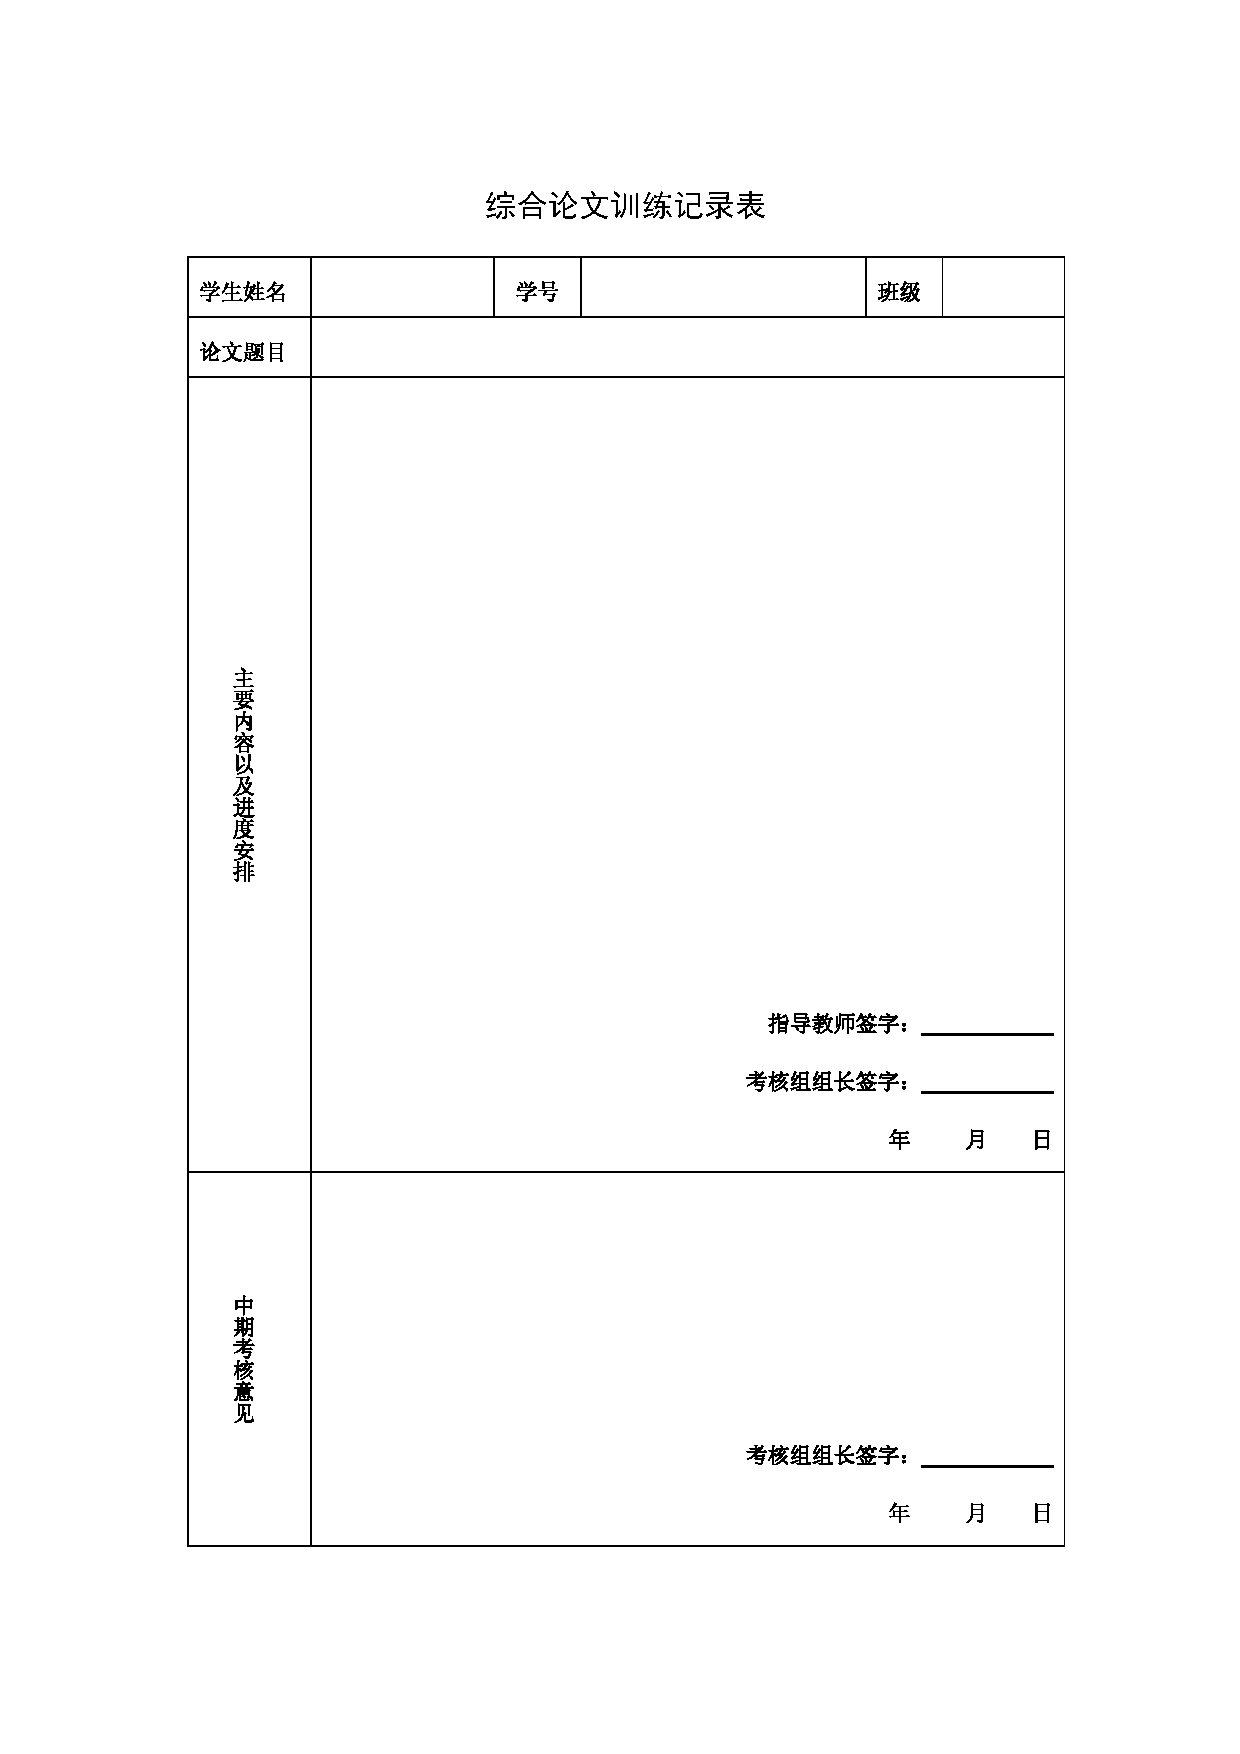
\includepdf[pages=-]{scan-record.pdf}
\end{document}
